\documentclass[1p]{elsarticle_modified}
%\bibliographystyle{elsarticle-num}

%\usepackage[colorlinks]{hyperref}
%\usepackage{abbrmath_seonhwa} %\Abb, \Ascr, \Acal ,\Abf, \Afrak
\usepackage{amsfonts}
\usepackage{amssymb}
\usepackage{amsmath}
\usepackage{amsthm}
\usepackage{scalefnt}
\usepackage{amsbsy}
\usepackage{kotex}
\usepackage{caption}
\usepackage{subfig}
\usepackage{color}
\usepackage{graphicx}
\usepackage{xcolor} %% white, black, red, green, blue, cyan, magenta, yellow
\usepackage{float}
\usepackage{setspace}
\usepackage{hyperref}

\usepackage{tikz}
\usetikzlibrary{arrows}

\usepackage{multirow}
\usepackage{array} % fixed length table
\usepackage{hhline}

%%%%%%%%%%%%%%%%%%%%%
\makeatletter
\renewcommand*\env@matrix[1][\arraystretch]{%
	\edef\arraystretch{#1}%
	\hskip -\arraycolsep
	\let\@ifnextchar\new@ifnextchar
	\array{*\c@MaxMatrixCols c}}
\makeatother %https://tex.stackexchange.com/questions/14071/how-can-i-increase-the-line-spacing-in-a-matrix
%%%%%%%%%%%%%%%

\usepackage[normalem]{ulem}

\newcommand{\msout}[1]{\ifmmode\text{\sout{\ensuremath{#1}}}\else\sout{#1}\fi}
%SOURCE: \msout is \stkout macro in https://tex.stackexchange.com/questions/20609/strikeout-in-math-mode

\newcommand{\cancel}[1]{
	\ifmmode
	{\color{red}\msout{#1}}
	\else
	{\color{red}\sout{#1}}
	\fi
}

\newcommand{\add}[1]{
	{\color{blue}\uwave{#1}}
}

\newcommand{\replace}[2]{
	\ifmmode
	{\color{red}\msout{#1}}{\color{blue}\uwave{#2}}
	\else
	{\color{red}\sout{#1}}{\color{blue}\uwave{#2}}
	\fi
}

\newcommand{\Sol}{\mathcal{S}} %segment
\newcommand{\D}{D} %diagram
\newcommand{\A}{\mathcal{A}} %arc


%%%%%%%%%%%%%%%%%%%%%%%%%%%%%5 test

\def\sl{\operatorname{\textup{SL}}(2,\Cbb)}
\def\psl{\operatorname{\textup{PSL}}(2,\Cbb)}
\def\quan{\mkern 1mu \triangleright \mkern 1mu}

\theoremstyle{definition}
\newtheorem{thm}{Theorem}[section]
\newtheorem{prop}[thm]{Proposition}
\newtheorem{lem}[thm]{Lemma}
\newtheorem{ques}[thm]{Question}
\newtheorem{cor}[thm]{Corollary}
\newtheorem{defn}[thm]{Definition}
\newtheorem{exam}[thm]{Example}
\newtheorem{rmk}[thm]{Remark}
\newtheorem{alg}[thm]{Algorithm}

\newcommand{\I}{\sqrt{-1}}
\begin{document}

%\begin{frontmatter}
%
%\title{Boundary parabolic representations of knots up to 8 crossings}
%
%%% Group authors per affiliation:
%\author{Yunhi Cho} 
%\address{Department of Mathematics, University of Seoul, Seoul, Korea}
%\ead{yhcho@uos.ac.kr}
%
%
%\author{Seonhwa Kim} %\fnref{s_kim}}
%\address{Center for Geometry and Physics, Institute for Basic Science, Pohang, 37673, Korea}
%\ead{ryeona17@ibs.re.kr}
%
%\author{Hyuk Kim}
%\address{Department of Mathematical Sciences, Seoul National University, Seoul 08826, Korea}
%\ead{hyukkim@snu.ac.kr}
%
%\author{Seokbeom Yoon}
%\address{Department of Mathematical Sciences, Seoul National University, Seoul, 08826,  Korea}
%\ead{sbyoon15@snu.ac.kr}
%
%\begin{abstract}
%We find all boundary parabolic representation of knots up to 8 crossings.
%
%\end{abstract}
%\begin{keyword}
%    \MSC[2010] 57M25 
%\end{keyword}
%
%\end{frontmatter}

%\linenumbers
%\tableofcontents
%
\newcommand\colored[1]{\textcolor{white}{\rule[-0.35ex]{0.8em}{1.4ex}}\kern-0.8em\color{red} #1}%
%\newcommand\colored[1]{\textcolor{white}{ #1}\kern-2.17ex	\textcolor{white}{ #1}\kern-1.81ex	\textcolor{white}{ #1}\kern-2.15ex\color{red}#1	}

{\Large $\underline{12a_{0480}~(K12a_{0480})}$}

\setlength{\tabcolsep}{10pt}
\renewcommand{\arraystretch}{1.6}
\vspace{1cm}\begin{tabular}{m{100pt}>{\centering\arraybackslash}m{274pt}}
\multirow{5}{120pt}{
	\centering
	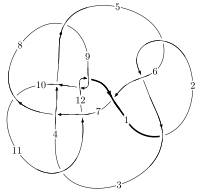
\includegraphics[width=112pt]{../../../GIT/diagram.site/Diagrams/png/1281_12a_0480.png}\\
\ \ \ A knot diagram\footnotemark}&
\allowdisplaybreaks
\textbf{Linearized knot diagam} \\
\cline{2-2}
 &
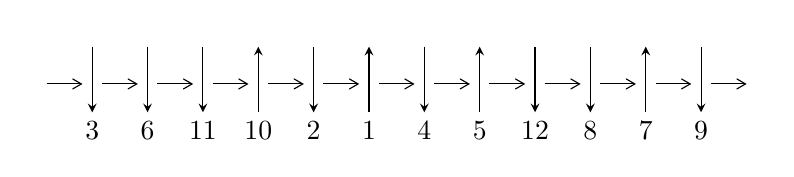
\begin{tikzpicture}[x=20pt, y=17pt]
	% nodes
	\node (C0) at (0, 0) {};
	\node (C1) at (1, 0) {};
	\node (C1U) at (1, +1) {};
	\node (C1D) at (1, -1) {3};

	\node (C2) at (2, 0) {};
	\node (C2U) at (2, +1) {};
	\node (C2D) at (2, -1) {6};

	\node (C3) at (3, 0) {};
	\node (C3U) at (3, +1) {};
	\node (C3D) at (3, -1) {11};

	\node (C4) at (4, 0) {};
	\node (C4U) at (4, +1) {};
	\node (C4D) at (4, -1) {10};

	\node (C5) at (5, 0) {};
	\node (C5U) at (5, +1) {};
	\node (C5D) at (5, -1) {2};

	\node (C6) at (6, 0) {};
	\node (C6U) at (6, +1) {};
	\node (C6D) at (6, -1) {1};

	\node (C7) at (7, 0) {};
	\node (C7U) at (7, +1) {};
	\node (C7D) at (7, -1) {4};

	\node (C8) at (8, 0) {};
	\node (C8U) at (8, +1) {};
	\node (C8D) at (8, -1) {5};

	\node (C9) at (9, 0) {};
	\node (C9U) at (9, +1) {};
	\node (C9D) at (9, -1) {12};

	\node (C10) at (10, 0) {};
	\node (C10U) at (10, +1) {};
	\node (C10D) at (10, -1) {8};

	\node (C11) at (11, 0) {};
	\node (C11U) at (11, +1) {};
	\node (C11D) at (11, -1) {7};

	\node (C12) at (12, 0) {};
	\node (C12U) at (12, +1) {};
	\node (C12D) at (12, -1) {9};
	\node (C13) at (13, 0) {};

	% arrows
	\draw[->,>={angle 60}]
	(C0) edge (C1) (C1) edge (C2) (C2) edge (C3) (C3) edge (C4) (C4) edge (C5) (C5) edge (C6) (C6) edge (C7) (C7) edge (C8) (C8) edge (C9) (C9) edge (C10) (C10) edge (C11) (C11) edge (C12) (C12) edge (C13) ;	\draw[->,>=stealth]
	(C1U) edge (C1D) (C2U) edge (C2D) (C3U) edge (C3D) (C4D) edge (C4U) (C5U) edge (C5D) (C6D) edge (C6U) (C7U) edge (C7D) (C8D) edge (C8U) (C9U) edge (C9D) (C10U) edge (C10D) (C11D) edge (C11U) (C12U) edge (C12D) ;
	\end{tikzpicture} \\
\hhline{~~} \\& 
\textbf{Solving Sequence} \\ \cline{2-2} 
 &
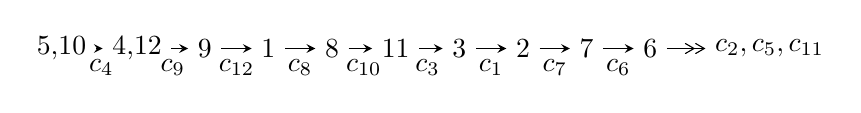
\begin{tikzpicture}[x=23pt, y=7pt]
	% node
	\node (A0) at (-1/8, 0) {5,10};
	\node (A1) at (17/16, 0) {4,12};
	\node (A2) at (17/8, 0) {9};
	\node (A3) at (25/8, 0) {1};
	\node (A4) at (33/8, 0) {8};
	\node (A5) at (41/8, 0) {11};
	\node (A6) at (49/8, 0) {3};
	\node (A7) at (57/8, 0) {2};
	\node (A8) at (65/8, 0) {7};
	\node (A9) at (73/8, 0) {6};
	\node (C1) at (1/2, -1) {$c_{4}$};
	\node (C2) at (13/8, -1) {$c_{9}$};
	\node (C3) at (21/8, -1) {$c_{12}$};
	\node (C4) at (29/8, -1) {$c_{8}$};
	\node (C5) at (37/8, -1) {$c_{10}$};
	\node (C6) at (45/8, -1) {$c_{3}$};
	\node (C7) at (53/8, -1) {$c_{1}$};
	\node (C8) at (61/8, -1) {$c_{7}$};
	\node (C9) at (69/8, -1) {$c_{6}$};
	\node (A10) at (11, 0) {$c_{2},c_{5},c_{11}$};

	% edge
	\draw[->,>=stealth]	
	(A0) edge (A1) (A1) edge (A2) (A2) edge (A3) (A3) edge (A4) (A4) edge (A5) (A5) edge (A6) (A6) edge (A7) (A7) edge (A8) (A8) edge (A9) ;
	\draw[->>,>={angle 60}]	
	(A9) edge (A10);
\end{tikzpicture} \\ 

\end{tabular} \\

\footnotetext{
The image of knot diagram is generated by the software ``\textbf{Draw programme}" developed by Andrew Bartholomew(\url{http://www.layer8.co.uk/maths/draw/index.htm\#Running-draw}), where we modified some parts for our purpose(\url{https://github.com/CATsTAILs/LinksPainter}).
}\phantom \\ \newline 
\centering \textbf{Ideals for irreducible components\footnotemark of $X_{\text{par}}$} 
 
\begin{align*}
I^u_{1}&=\langle 
-5.53974\times10^{1782} u^{185}-1.04886\times10^{1782} u^{184}+\cdots+1.94118\times10^{1786} b-1.46314\times10^{1786},\\
\phantom{I^u_{1}}&\phantom{= \langle  }-2.97721\times10^{1785} u^{185}+6.39771\times10^{1785} u^{184}+\cdots+2.13529\times10^{1787} a+1.77330\times10^{1787},\\
\phantom{I^u_{1}}&\phantom{= \langle  }u^{186}-2 u^{185}+\cdots+36 u+88\rangle \\
I^u_{2}&=\langle 
-2.01366\times10^{18} u^{38}-2.85310\times10^{18} u^{37}+\cdots+3.17258\times10^{16} b+5.50245\times10^{18},\\
\phantom{I^u_{2}}&\phantom{= \langle  }-1.58873\times10^{18} u^{38}-1.90932\times10^{18} u^{37}+\cdots+3.17258\times10^{16} a+3.87866\times10^{18},\;u^{39}-8 u^{37}+\cdots- u+1\rangle \\
I^u_{3}&=\langle 
- u^3- u^2+b-3 u,\;- u^3+a-2 u+1,\;u^4+u^3+3 u^2+u+1\rangle \\
\\
\end{align*}
\raggedright * 3 irreducible components of $\dim_{\mathbb{C}}=0$, with total 229 representations.\\
\footnotetext{All coefficients of polynomials are rational numbers. But the coefficients are sometimes approximated in decimal forms when there is not enough margin.}
\newpage
\renewcommand{\arraystretch}{1}
\centering \section*{I. $I^u_{1}= \langle -5.54\times10^{1782} u^{185}-1.05\times10^{1782} u^{184}+\cdots+1.94\times10^{1786} b-1.46\times10^{1786},\;-2.98\times10^{1785} u^{185}+6.40\times10^{1785} u^{184}+\cdots+2.14\times10^{1787} a+1.77\times10^{1787},\;u^{186}-2 u^{185}+\cdots+36 u+88 \rangle$}
\flushleft \textbf{(i) Arc colorings}\\
\begin{tabular}{m{7pt} m{180pt} m{7pt} m{180pt} }
\flushright $a_{5}=$&$\begin{pmatrix}1\\0\end{pmatrix}$ \\
\flushright $a_{10}=$&$\begin{pmatrix}0\\u\end{pmatrix}$ \\
\flushright $a_{4}=$&$\begin{pmatrix}1\\u^2\end{pmatrix}$ \\
\flushright $a_{12}=$&$\begin{pmatrix}0.0139429 u^{185}-0.0299617 u^{184}+\cdots+27.9469 u-0.830473\\0.000285381 u^{185}+0.0000540324 u^{184}+\cdots-3.59654 u+0.753738\end{pmatrix}$ \\
\flushright $a_{9}=$&$\begin{pmatrix}-0.0142463 u^{185}+0.0252800 u^{184}+\cdots-20.5127 u-1.57779\\-0.00499165 u^{185}+0.0105584 u^{184}+\cdots+3.21433 u-1.41591\end{pmatrix}$ \\
\flushright $a_{1}=$&$\begin{pmatrix}0.0267348 u^{185}-0.0563542 u^{184}+\cdots+62.5196 u-4.69174\\-0.00716177 u^{185}+0.0148747 u^{184}+\cdots-6.57632 u-1.44609\end{pmatrix}$ \\
\flushright $a_{8}=$&$\begin{pmatrix}-0.00925466 u^{185}+0.0147216 u^{184}+\cdots-23.7270 u-0.161882\\-0.00499165 u^{185}+0.0105584 u^{184}+\cdots+3.21433 u-1.41591\end{pmatrix}$ \\
\flushright $a_{11}=$&$\begin{pmatrix}0.0282924 u^{185}-0.0611872 u^{184}+\cdots+48.9451 u-4.17978\\-0.00392221 u^{185}+0.00742383 u^{184}+\cdots-5.18728 u-0.958823\end{pmatrix}$ \\
\flushright $a_{3}=$&$\begin{pmatrix}0.0381994 u^{185}-0.0873826 u^{184}+\cdots+22.1562 u-17.5234\\-0.00538202 u^{185}+0.0115863 u^{184}+\cdots-4.88044 u-0.286897\end{pmatrix}$ \\
\flushright $a_{2}=$&$\begin{pmatrix}-0.0408306 u^{185}+0.0758692 u^{184}+\cdots-42.0542 u-6.21348\\-0.000658012 u^{185}+0.00163785 u^{184}+\cdots-1.35113 u+0.743251\end{pmatrix}$ \\
\flushright $a_{7}=$&$\begin{pmatrix}-0.0152408 u^{185}+0.0271515 u^{184}+\cdots-21.4634 u-1.91111\\-0.00417663 u^{185}+0.00854602 u^{184}+\cdots+3.72464 u-1.45617\end{pmatrix}$ \\
\flushright $a_{6}=$&$\begin{pmatrix}-0.0311906 u^{185}+0.0491555 u^{184}+\cdots-44.2840 u-15.9001\\-0.00170698 u^{185}+0.00411396 u^{184}+\cdots-3.64158 u+1.07199\end{pmatrix}$\\&\end{tabular}
\flushleft \textbf{(ii) Obstruction class $= -1$}\\~\\
\flushleft \textbf{(iii) Cusp Shapes $= -0.0273306 u^{185}+0.0429325 u^{184}+\cdots+5.94117 u-29.4743$}\\~\\
\newpage\renewcommand{\arraystretch}{1}
\flushleft \textbf{(iv) u-Polynomials at the component}\newline \\
\begin{tabular}{m{50pt}|m{274pt}}
Crossings & \hspace{64pt}u-Polynomials at each crossing \\
\hline $$\begin{aligned}c_{1}\end{aligned}$$&$\begin{aligned}
&u^{186}+93 u^{185}+\cdots+190 u+1
\end{aligned}$\\
\hline $$\begin{aligned}c_{2},c_{5}\end{aligned}$$&$\begin{aligned}
&u^{186}+u^{185}+\cdots+10 u-1
\end{aligned}$\\
\hline $$\begin{aligned}c_{3}\end{aligned}$$&$\begin{aligned}
&u^{186}+5 u^{185}+\cdots+305 u+29
\end{aligned}$\\
\hline $$\begin{aligned}c_{4}\end{aligned}$$&$\begin{aligned}
&u^{186}+2 u^{185}+\cdots-36 u+88
\end{aligned}$\\
\hline $$\begin{aligned}c_{6}\end{aligned}$$&$\begin{aligned}
&u^{186}-9 u^{185}+\cdots+133392896 u-8998912
\end{aligned}$\\
\hline $$\begin{aligned}c_{7}\end{aligned}$$&$\begin{aligned}
&u^{186}+4 u^{185}+\cdots+96 u-17
\end{aligned}$\\
\hline $$\begin{aligned}c_{8}\end{aligned}$$&$\begin{aligned}
&u^{186}+3 u^{185}+\cdots+264890731 u+56493497
\end{aligned}$\\
\hline $$\begin{aligned}c_{9},c_{12}\end{aligned}$$&$\begin{aligned}
&u^{186}+11 u^{185}+\cdots+2925 u+459
\end{aligned}$\\
\hline $$\begin{aligned}c_{10}\end{aligned}$$&$\begin{aligned}
&u^{186}-12 u^{185}+\cdots+104 u-16
\end{aligned}$\\
\hline $$\begin{aligned}c_{11}\end{aligned}$$&$\begin{aligned}
&u^{186}-3 u^{185}+\cdots+2837302 u+121613
\end{aligned}$\\
\hline
\end{tabular}\\~\\
\newpage\renewcommand{\arraystretch}{1}
\flushleft \textbf{(v) Riley Polynomials at the component}\newline \\
\begin{tabular}{m{50pt}|m{274pt}}
Crossings & \hspace{64pt}Riley Polynomials at each crossing \\
\hline $$\begin{aligned}c_{1}\end{aligned}$$&$\begin{aligned}
&y^{186}+15 y^{185}+\cdots-32898 y+1
\end{aligned}$\\
\hline $$\begin{aligned}c_{2},c_{5}\end{aligned}$$&$\begin{aligned}
&y^{186}-93 y^{185}+\cdots-190 y+1
\end{aligned}$\\
\hline $$\begin{aligned}c_{3}\end{aligned}$$&$\begin{aligned}
&y^{186}- y^{185}+\cdots+166641 y+841
\end{aligned}$\\
\hline $$\begin{aligned}c_{4}\end{aligned}$$&$\begin{aligned}
&y^{186}-4 y^{185}+\cdots+366192 y+7744
\end{aligned}$\\
\hline $$\begin{aligned}c_{6}\end{aligned}$$&$\begin{aligned}
&y^{186}+51 y^{185}+\cdots-15721607766212608 y+80980417183744
\end{aligned}$\\
\hline $$\begin{aligned}c_{7}\end{aligned}$$&$\begin{aligned}
&y^{186}-6 y^{185}+\cdots-20878 y+289
\end{aligned}$\\
\hline $$\begin{aligned}c_{8}\end{aligned}$$&$\begin{aligned}
&y^{186}-21 y^{185}+\cdots-86383388203073361 y+3191515203289009
\end{aligned}$\\
\hline $$\begin{aligned}c_{9},c_{12}\end{aligned}$$&$\begin{aligned}
&y^{186}+101 y^{185}+\cdots-66119733 y+210681
\end{aligned}$\\
\hline $$\begin{aligned}c_{10}\end{aligned}$$&$\begin{aligned}
&y^{186}+2 y^{185}+\cdots+15552 y+256
\end{aligned}$\\
\hline $$\begin{aligned}c_{11}\end{aligned}$$&$\begin{aligned}
&y^{186}+y^{185}+\cdots+730297573796 y+14789721769
\end{aligned}$\\
\hline
\end{tabular}\\~\\
\newpage\flushleft \textbf{(vi) Complex Volumes and Cusp Shapes}
$$\begin{array}{c|c|c}  
\text{Solutions to }I^u_{1}& \I (\text{vol} + \sqrt{-1}CS) & \text{Cusp shape}\\
 \hline 
\begin{aligned}
u &= -0.307193 + 0.967341 I \\
a &= \phantom{-}0.781942 - 0.330599 I \\
b &= \phantom{-}1.066600 - 0.168179 I\end{aligned}
 & \phantom{-}0.97519 - 5.05662 I & \phantom{-0.000000 } 0 \\ \hline\begin{aligned}
u &= -0.307193 - 0.967341 I \\
a &= \phantom{-}0.781942 + 0.330599 I \\
b &= \phantom{-}1.066600 + 0.168179 I\end{aligned}
 & \phantom{-}0.97519 + 5.05662 I & \phantom{-0.000000 } 0 \\ \hline\begin{aligned}
u &= \phantom{-}0.253390 + 0.990747 I \\
a &= -0.242638 + 0.284026 I \\
b &= \phantom{-}0.380788 + 0.645948 I\end{aligned}
 & -1.86439 - 1.17440 I & \phantom{-0.000000 } 0 \\ \hline\begin{aligned}
u &= \phantom{-}0.253390 - 0.990747 I \\
a &= -0.242638 - 0.284026 I \\
b &= \phantom{-}0.380788 - 0.645948 I\end{aligned}
 & -1.86439 + 1.17440 I & \phantom{-0.000000 } 0 \\ \hline\begin{aligned}
u &= -0.675127 + 0.780576 I \\
a &= -0.613719 + 1.037810 I \\
b &= \phantom{-}1.07465 + 2.13225 I\end{aligned}
 & \phantom{-}2.11722 - 10.27940 I & \phantom{-0.000000 } 0 \\ \hline\begin{aligned}
u &= -0.675127 - 0.780576 I \\
a &= -0.613719 - 1.037810 I \\
b &= \phantom{-}1.07465 - 2.13225 I\end{aligned}
 & \phantom{-}2.11722 + 10.27940 I & \phantom{-0.000000 } 0 \\ \hline\begin{aligned}
u &= \phantom{-}0.853275 + 0.452540 I \\
a &= -0.088030 - 1.280050 I \\
b &= \phantom{-}0.45272 - 2.29319 I\end{aligned}
 & \phantom{-}3.49418 + 6.86248 I & \phantom{-0.000000 } 0 \\ \hline\begin{aligned}
u &= \phantom{-}0.853275 - 0.452540 I \\
a &= -0.088030 + 1.280050 I \\
b &= \phantom{-}0.45272 + 2.29319 I\end{aligned}
 & \phantom{-}3.49418 - 6.86248 I & \phantom{-0.000000 } 0 \\ \hline\begin{aligned}
u &= -0.804997 + 0.530431 I \\
a &= \phantom{-}0.171471 - 1.314710 I \\
b &= -0.40826 - 2.32898 I\end{aligned}
 & \phantom{-}0.91102 - 12.26790 I & \phantom{-0.000000 } 0 \\ \hline\begin{aligned}
u &= -0.804997 - 0.530431 I \\
a &= \phantom{-}0.171471 + 1.314710 I \\
b &= -0.40826 + 2.32898 I\end{aligned}
 & \phantom{-}0.91102 + 12.26790 I & \phantom{-0.000000 } 0\\
 \hline 
 \end{array}$$\newpage$$\begin{array}{c|c|c}  
\text{Solutions to }I^u_{1}& \I (\text{vol} + \sqrt{-1}CS) & \text{Cusp shape}\\
 \hline 
\begin{aligned}
u &= \phantom{-}0.083825 + 0.956958 I \\
a &= -1.119070 - 0.433268 I \\
b &= -1.258870 - 0.213178 I\end{aligned}
 & -2.73445 + 10.40150 I & \phantom{-0.000000 } 0 \\ \hline\begin{aligned}
u &= \phantom{-}0.083825 - 0.956958 I \\
a &= -1.119070 + 0.433268 I \\
b &= -1.258870 + 0.213178 I\end{aligned}
 & -2.73445 - 10.40150 I & \phantom{-0.000000 } 0 \\ \hline\begin{aligned}
u &= -0.674689 + 0.681706 I \\
a &= -0.598741 + 0.989226 I \\
b &= \phantom{-}1.28601 + 1.91959 I\end{aligned}
 & \phantom{-}0.76354 - 2.80393 I & \phantom{-0.000000 } 0 \\ \hline\begin{aligned}
u &= -0.674689 - 0.681706 I \\
a &= -0.598741 - 0.989226 I \\
b &= \phantom{-}1.28601 - 1.91959 I\end{aligned}
 & \phantom{-}0.76354 + 2.80393 I & \phantom{-0.000000 } 0 \\ \hline\begin{aligned}
u &= \phantom{-}0.437848 + 0.842864 I \\
a &= \phantom{-}0.147642 + 1.039510 I \\
b &= -0.577907 + 0.605984 I\end{aligned}
 & -2.56560 - 3.06621 I & \phantom{-0.000000 } 0 \\ \hline\begin{aligned}
u &= \phantom{-}0.437848 - 0.842864 I \\
a &= \phantom{-}0.147642 - 1.039510 I \\
b &= -0.577907 - 0.605984 I\end{aligned}
 & -2.56560 + 3.06621 I & \phantom{-0.000000 } 0 \\ \hline\begin{aligned}
u &= \phantom{-}0.717695 + 0.768921 I \\
a &= \phantom{-}0.633626 + 1.017910 I \\
b &= -1.02258 + 2.01828 I\end{aligned}
 & \phantom{-}4.47017 + 5.65374 I & \phantom{-0.000000 } 0 \\ \hline\begin{aligned}
u &= \phantom{-}0.717695 - 0.768921 I \\
a &= \phantom{-}0.633626 - 1.017910 I \\
b &= -1.02258 - 2.01828 I\end{aligned}
 & \phantom{-}4.47017 - 5.65374 I & \phantom{-0.000000 } 0 \\ \hline\begin{aligned}
u &= \phantom{-}1.012420 + 0.307233 I \\
a &= -1.199850 + 0.186361 I \\
b &= \phantom{-}0.364057 - 0.040225 I\end{aligned}
 & -2.46023 + 0.04685 I & \phantom{-0.000000 } 0 \\ \hline\begin{aligned}
u &= \phantom{-}1.012420 - 0.307233 I \\
a &= -1.199850 - 0.186361 I \\
b &= \phantom{-}0.364057 + 0.040225 I\end{aligned}
 & -2.46023 - 0.04685 I & \phantom{-0.000000 } 0\\
 \hline 
 \end{array}$$\newpage$$\begin{array}{c|c|c}  
\text{Solutions to }I^u_{1}& \I (\text{vol} + \sqrt{-1}CS) & \text{Cusp shape}\\
 \hline 
\begin{aligned}
u &= \phantom{-}0.572390 + 0.897115 I \\
a &= -0.663827 + 0.353353 I \\
b &= \phantom{-}0.133217 + 1.285900 I\end{aligned}
 & -0.80538 - 2.62868 I & \phantom{-0.000000 } 0 \\ \hline\begin{aligned}
u &= \phantom{-}0.572390 - 0.897115 I \\
a &= -0.663827 - 0.353353 I \\
b &= \phantom{-}0.133217 - 1.285900 I\end{aligned}
 & -0.80538 + 2.62868 I & \phantom{-0.000000 } 0 \\ \hline\begin{aligned}
u &= -0.354982 + 0.861592 I \\
a &= -0.305662 + 0.873306 I \\
b &= \phantom{-}0.413471 + 0.524540 I\end{aligned}
 & -0.32060 - 1.51914 I & \phantom{-0.000000 } 0 \\ \hline\begin{aligned}
u &= -0.354982 - 0.861592 I \\
a &= -0.305662 - 0.873306 I \\
b &= \phantom{-}0.413471 - 0.524540 I\end{aligned}
 & -0.32060 + 1.51914 I & \phantom{-0.000000 } 0 \\ \hline\begin{aligned}
u &= -0.722798 + 0.788914 I \\
a &= -0.257287 - 0.728218 I \\
b &= \phantom{-}0.363899 - 0.423076 I\end{aligned}
 & \phantom{-}0.55644 - 3.03027 I & \phantom{-0.000000 } 0 \\ \hline\begin{aligned}
u &= -0.722798 - 0.788914 I \\
a &= -0.257287 + 0.728218 I \\
b &= \phantom{-}0.363899 + 0.423076 I\end{aligned}
 & \phantom{-}0.55644 + 3.03027 I & \phantom{-0.000000 } 0 \\ \hline\begin{aligned}
u &= -0.096124 + 1.069100 I \\
a &= -0.601379 + 0.578893 I \\
b &= \phantom{-}0.467546 - 0.017428 I\end{aligned}
 & -0.06484 - 3.30755 I & \phantom{-0.000000 } 0 \\ \hline\begin{aligned}
u &= -0.096124 - 1.069100 I \\
a &= -0.601379 - 0.578893 I \\
b &= \phantom{-}0.467546 + 0.017428 I\end{aligned}
 & -0.06484 + 3.30755 I & \phantom{-0.000000 } 0 \\ \hline\begin{aligned}
u &= -0.138168 + 0.909744 I \\
a &= \phantom{-}1.045970 - 0.490376 I \\
b &= \phantom{-}1.224420 - 0.250675 I\end{aligned}
 & -0.19438 - 5.76200 I & \phantom{-0.000000 } 0 \\ \hline\begin{aligned}
u &= -0.138168 - 0.909744 I \\
a &= \phantom{-}1.045970 + 0.490376 I \\
b &= \phantom{-}1.224420 + 0.250675 I\end{aligned}
 & -0.19438 + 5.76200 I & \phantom{-0.000000 } 0\\
 \hline 
 \end{array}$$\newpage$$\begin{array}{c|c|c}  
\text{Solutions to }I^u_{1}& \I (\text{vol} + \sqrt{-1}CS) & \text{Cusp shape}\\
 \hline 
\begin{aligned}
u &= -0.059355 + 1.086540 I \\
a &= \phantom{-}0.788852 + 0.515087 I \\
b &= -0.458485 - 0.205965 I\end{aligned}
 & -1.89169 + 8.37857 I & \phantom{-0.000000 } 0 \\ \hline\begin{aligned}
u &= -0.059355 - 1.086540 I \\
a &= \phantom{-}0.788852 - 0.515087 I \\
b &= -0.458485 + 0.205965 I\end{aligned}
 & -1.89169 - 8.37857 I & \phantom{-0.000000 } 0 \\ \hline\begin{aligned}
u &= \phantom{-}0.363478 + 1.028510 I \\
a &= -0.731178 - 0.148405 I \\
b &= -1.038010 - 0.061869 I\end{aligned}
 & -0.537922 + 1.129420 I & \phantom{-0.000000 } 0 \\ \hline\begin{aligned}
u &= \phantom{-}0.363478 - 1.028510 I \\
a &= -0.731178 + 0.148405 I \\
b &= -1.038010 + 0.061869 I\end{aligned}
 & -0.537922 - 1.129420 I & \phantom{-0.000000 } 0 \\ \hline\begin{aligned}
u &= \phantom{-}0.824270 + 0.374120 I \\
a &= \phantom{-}0.639506 + 0.965348 I \\
b &= -1.02094 + 1.02954 I\end{aligned}
 & \phantom{-}1.83442 + 4.12238 I & \phantom{-0.000000 } 0 \\ \hline\begin{aligned}
u &= \phantom{-}0.824270 - 0.374120 I \\
a &= \phantom{-}0.639506 - 0.965348 I \\
b &= -1.02094 - 1.02954 I\end{aligned}
 & \phantom{-}1.83442 - 4.12238 I & \phantom{-0.000000 } 0 \\ \hline\begin{aligned}
u &= -0.314606 + 0.829544 I \\
a &= -0.444797 + 0.667757 I \\
b &= \phantom{-}0.092191 + 0.608271 I\end{aligned}
 & -0.38674 - 1.57867 I & \phantom{-0.000000 } 0 \\ \hline\begin{aligned}
u &= -0.314606 - 0.829544 I \\
a &= -0.444797 - 0.667757 I \\
b &= \phantom{-}0.092191 - 0.608271 I\end{aligned}
 & -0.38674 + 1.57867 I & \phantom{-0.000000 } 0 \\ \hline\begin{aligned}
u &= \phantom{-}0.461175 + 1.019950 I \\
a &= -0.443544 + 0.006626 I \\
b &= -0.877062 + 0.035310 I\end{aligned}
 & -0.59177 + 7.29260 I & \phantom{-0.000000 } 0 \\ \hline\begin{aligned}
u &= \phantom{-}0.461175 - 1.019950 I \\
a &= -0.443544 - 0.006626 I \\
b &= -0.877062 - 0.035310 I\end{aligned}
 & -0.59177 - 7.29260 I & \phantom{-0.000000 } 0\\
 \hline 
 \end{array}$$\newpage$$\begin{array}{c|c|c}  
\text{Solutions to }I^u_{1}& \I (\text{vol} + \sqrt{-1}CS) & \text{Cusp shape}\\
 \hline 
\begin{aligned}
u &= -0.178724 + 1.105860 I \\
a &= -0.807341 + 0.478053 I \\
b &= -0.069089 + 0.893742 I\end{aligned}
 & \phantom{-}0.16929 - 1.66192 I & \phantom{-0.000000 } 0 \\ \hline\begin{aligned}
u &= -0.178724 - 1.105860 I \\
a &= -0.807341 - 0.478053 I \\
b &= -0.069089 - 0.893742 I\end{aligned}
 & \phantom{-}0.16929 + 1.66192 I & \phantom{-0.000000 } 0 \\ \hline\begin{aligned}
u &= \phantom{-}0.180928 + 1.107630 I \\
a &= -0.837168 + 0.470067 I \\
b &= -0.052148 + 1.106190 I\end{aligned}
 & \phantom{-}0.20180 - 2.41331 I & \phantom{-0.000000 } 0 \\ \hline\begin{aligned}
u &= \phantom{-}0.180928 - 1.107630 I \\
a &= -0.837168 - 0.470067 I \\
b &= -0.052148 - 1.106190 I\end{aligned}
 & \phantom{-}0.20180 + 2.41331 I & \phantom{-0.000000 } 0 \\ \hline\begin{aligned}
u &= \phantom{-}0.645795 + 0.586749 I \\
a &= \phantom{-}0.900189 - 0.344371 I \\
b &= \phantom{-}0.662748 + 0.097500 I\end{aligned}
 & -1.59920 + 7.23039 I & \phantom{-0.000000 } 0 \\ \hline\begin{aligned}
u &= \phantom{-}0.645795 - 0.586749 I \\
a &= \phantom{-}0.900189 + 0.344371 I \\
b &= \phantom{-}0.662748 - 0.097500 I\end{aligned}
 & -1.59920 - 7.23039 I & \phantom{-0.000000 } 0 \\ \hline\begin{aligned}
u &= \phantom{-}1.118920 + 0.235863 I \\
a &= \phantom{-}0.662261 + 1.001360 I \\
b &= -0.425293 + 1.057500 I\end{aligned}
 & \phantom{-}3.68148 - 2.29871 I & \phantom{-0.000000 } 0 \\ \hline\begin{aligned}
u &= \phantom{-}1.118920 - 0.235863 I \\
a &= \phantom{-}0.662261 - 1.001360 I \\
b &= -0.425293 - 1.057500 I\end{aligned}
 & \phantom{-}3.68148 + 2.29871 I & \phantom{-0.000000 } 0 \\ \hline\begin{aligned}
u &= \phantom{-}0.793640 + 0.825156 I \\
a &= \phantom{-}0.695600 + 0.985737 I \\
b &= -0.80313 + 1.93853 I\end{aligned}
 & \phantom{-}5.36288 + 4.49134 I & \phantom{-0.000000 } 0 \\ \hline\begin{aligned}
u &= \phantom{-}0.793640 - 0.825156 I \\
a &= \phantom{-}0.695600 - 0.985737 I \\
b &= -0.80313 - 1.93853 I\end{aligned}
 & \phantom{-}5.36288 - 4.49134 I & \phantom{-0.000000 } 0\\
 \hline 
 \end{array}$$\newpage$$\begin{array}{c|c|c}  
\text{Solutions to }I^u_{1}& \I (\text{vol} + \sqrt{-1}CS) & \text{Cusp shape}\\
 \hline 
\begin{aligned}
u &= -0.547707 + 1.009050 I \\
a &= \phantom{-}0.0232921 - 0.0858861 I \\
b &= \phantom{-}0.626031 + 0.023105 I\end{aligned}
 & \phantom{-}0.64769 - 3.32832 I & \phantom{-0.000000 } 0 \\ \hline\begin{aligned}
u &= -0.547707 - 1.009050 I \\
a &= \phantom{-}0.0232921 + 0.0858861 I \\
b &= \phantom{-}0.626031 - 0.023105 I\end{aligned}
 & \phantom{-}0.64769 + 3.32832 I & \phantom{-0.000000 } 0 \\ \hline\begin{aligned}
u &= -0.854073 + 0.774154 I \\
a &= \phantom{-}0.467182 + 0.340599 I \\
b &= -0.31259 + 1.45543 I\end{aligned}
 & -4.49622 - 0.82832 I & \phantom{-0.000000 } 0 \\ \hline\begin{aligned}
u &= -0.854073 - 0.774154 I \\
a &= \phantom{-}0.467182 - 0.340599 I \\
b &= -0.31259 - 1.45543 I\end{aligned}
 & -4.49622 + 0.82832 I & \phantom{-0.000000 } 0 \\ \hline\begin{aligned}
u &= \phantom{-}0.408699 + 0.733043 I \\
a &= \phantom{-}0.422778 + 1.292510 I \\
b &= -0.518609 + 0.803977 I\end{aligned}
 & -3.93842 + 4.35538 I & \phantom{-0.000000 } 0 \\ \hline\begin{aligned}
u &= \phantom{-}0.408699 - 0.733043 I \\
a &= \phantom{-}0.422778 - 1.292510 I \\
b &= -0.518609 - 0.803977 I\end{aligned}
 & -3.93842 - 4.35538 I & \phantom{-0.000000 } 0 \\ \hline\begin{aligned}
u &= -1.124830 + 0.340404 I \\
a &= -0.641335 + 1.005070 I \\
b &= \phantom{-}0.497320 + 1.184150 I\end{aligned}
 & \phantom{-}5.59008 - 2.33345 I & \phantom{-0.000000 } 0 \\ \hline\begin{aligned}
u &= -1.124830 - 0.340404 I \\
a &= -0.641335 - 1.005070 I \\
b &= \phantom{-}0.497320 - 1.184150 I\end{aligned}
 & \phantom{-}5.59008 + 2.33345 I & \phantom{-0.000000 } 0 \\ \hline\begin{aligned}
u &= \phantom{-}0.037545 + 0.823907 I \\
a &= -1.200190 - 0.581568 I \\
b &= -1.326440 - 0.283115 I\end{aligned}
 & -4.04651 + 2.52728 I & \phantom{-0.000000 } 0 \\ \hline\begin{aligned}
u &= \phantom{-}0.037545 - 0.823907 I \\
a &= -1.200190 + 0.581568 I \\
b &= -1.326440 + 0.283115 I\end{aligned}
 & -4.04651 - 2.52728 I & \phantom{-0.000000 } 0\\
 \hline 
 \end{array}$$\newpage$$\begin{array}{c|c|c}  
\text{Solutions to }I^u_{1}& \I (\text{vol} + \sqrt{-1}CS) & \text{Cusp shape}\\
 \hline 
\begin{aligned}
u &= -0.621603 + 0.537572 I \\
a &= -0.786093 - 0.301539 I \\
b &= -0.552595 + 0.187397 I\end{aligned}
 & \phantom{-}0.92510 - 2.38169 I & \phantom{-0.000000 } 0 \\ \hline\begin{aligned}
u &= -0.621603 - 0.537572 I \\
a &= -0.786093 + 0.301539 I \\
b &= -0.552595 - 0.187397 I\end{aligned}
 & \phantom{-}0.92510 + 2.38169 I & \phantom{-0.000000 } 0 \\ \hline\begin{aligned}
u &= -0.802130 + 0.868304 I \\
a &= -0.750133 + 0.960332 I \\
b &= \phantom{-}0.70462 + 1.93410 I\end{aligned}
 & \phantom{-}3.90480 - 0.23906 I & \phantom{-0.000000 } 0 \\ \hline\begin{aligned}
u &= -0.802130 - 0.868304 I \\
a &= -0.750133 - 0.960332 I \\
b &= \phantom{-}0.70462 - 1.93410 I\end{aligned}
 & \phantom{-}3.90480 + 0.23906 I & \phantom{-0.000000 } 0 \\ \hline\begin{aligned}
u &= -0.002919 + 0.805198 I \\
a &= \phantom{-}0.815890 + 1.030460 I \\
b &= -0.121074 - 0.105187 I\end{aligned}
 & -4.49936 + 1.46905 I & \phantom{-0.000000 } 0 \\ \hline\begin{aligned}
u &= -0.002919 - 0.805198 I \\
a &= \phantom{-}0.815890 - 1.030460 I \\
b &= -0.121074 + 0.105187 I\end{aligned}
 & -4.49936 - 1.46905 I & \phantom{-0.000000 } 0 \\ \hline\begin{aligned}
u &= \phantom{-}0.555168 + 0.572524 I \\
a &= \phantom{-}0.953028 - 0.052468 I \\
b &= \phantom{-}0.794971 + 0.426716 I\end{aligned}
 & -3.23830 - 0.80541 I & \phantom{-0.000000 } 0 \\ \hline\begin{aligned}
u &= \phantom{-}0.555168 - 0.572524 I \\
a &= \phantom{-}0.953028 + 0.052468 I \\
b &= \phantom{-}0.794971 - 0.426716 I\end{aligned}
 & -3.23830 + 0.80541 I & \phantom{-0.000000 } 0 \\ \hline\begin{aligned}
u &= -0.715525 + 0.305973 I \\
a &= -0.07814 - 1.46534 I \\
b &= -0.58982 - 2.36264 I\end{aligned}
 & -1.71930 - 3.48624 I & \phantom{-0.000000 } 0 \\ \hline\begin{aligned}
u &= -0.715525 - 0.305973 I \\
a &= -0.07814 + 1.46534 I \\
b &= -0.58982 + 2.36264 I\end{aligned}
 & -1.71930 + 3.48624 I & \phantom{-0.000000 } 0\\
 \hline 
 \end{array}$$\newpage$$\begin{array}{c|c|c}  
\text{Solutions to }I^u_{1}& \I (\text{vol} + \sqrt{-1}CS) & \text{Cusp shape}\\
 \hline 
\begin{aligned}
u &= -0.293268 + 1.195460 I \\
a &= -0.670844 + 0.095073 I \\
b &= \phantom{-}0.60534 + 1.50815 I\end{aligned}
 & \phantom{-}0.93337 + 5.95821 I & \phantom{-0.000000 } 0 \\ \hline\begin{aligned}
u &= -0.293268 - 1.195460 I \\
a &= -0.670844 - 0.095073 I \\
b &= \phantom{-}0.60534 - 1.50815 I\end{aligned}
 & \phantom{-}0.93337 - 5.95821 I & \phantom{-0.000000 } 0 \\ \hline\begin{aligned}
u &= \phantom{-}0.765582\phantom{ +0.000000I} \\
a &= -1.59013\phantom{ +0.000000I} \\
b &= \phantom{-}0.345767\phantom{ +0.000000I}\end{aligned}
 & -2.40105\phantom{ +0.000000I} & \phantom{-0.000000 } 0 \\ \hline\begin{aligned}
u &= \phantom{-}1.227480 + 0.151731 I \\
a &= \phantom{-}0.113179 - 0.892273 I \\
b &= \phantom{-}0.44000 - 2.10931 I\end{aligned}
 & \phantom{-}6.17978 + 3.50042 I & \phantom{-0.000000 } 0 \\ \hline\begin{aligned}
u &= \phantom{-}1.227480 - 0.151731 I \\
a &= \phantom{-}0.113179 + 0.892273 I \\
b &= \phantom{-}0.44000 + 2.10931 I\end{aligned}
 & \phantom{-}6.17978 - 3.50042 I & \phantom{-0.000000 } 0 \\ \hline\begin{aligned}
u &= \phantom{-}0.846541 + 0.902891 I \\
a &= \phantom{-}0.518287 - 0.568193 I \\
b &= -0.138262 - 0.293557 I\end{aligned}
 & \phantom{-}1.13484 + 7.43949 I & \phantom{-0.000000 } 0 \\ \hline\begin{aligned}
u &= \phantom{-}0.846541 - 0.902891 I \\
a &= \phantom{-}0.518287 + 0.568193 I \\
b &= -0.138262 + 0.293557 I\end{aligned}
 & \phantom{-}1.13484 - 7.43949 I & \phantom{-0.000000 } 0 \\ \hline\begin{aligned}
u &= -0.682853 + 1.040320 I \\
a &= \phantom{-}0.618865 + 0.451464 I \\
b &= -0.066563 + 1.392200 I\end{aligned}
 & -3.46205 + 7.14168 I & \phantom{-0.000000 } 0 \\ \hline\begin{aligned}
u &= -0.682853 - 1.040320 I \\
a &= \phantom{-}0.618865 - 0.451464 I \\
b &= -0.066563 - 1.392200 I\end{aligned}
 & -3.46205 - 7.14168 I & \phantom{-0.000000 } 0 \\ \hline\begin{aligned}
u &= -0.639613 + 0.337366 I \\
a &= -0.499949 - 0.582165 I \\
b &= -0.141593 + 0.133008 I\end{aligned}
 & \phantom{-}2.53289 - 0.95957 I & \phantom{-0.000000 } 0\\
 \hline 
 \end{array}$$\newpage$$\begin{array}{c|c|c}  
\text{Solutions to }I^u_{1}& \I (\text{vol} + \sqrt{-1}CS) & \text{Cusp shape}\\
 \hline 
\begin{aligned}
u &= -0.639613 - 0.337366 I \\
a &= -0.499949 + 0.582165 I \\
b &= -0.141593 - 0.133008 I\end{aligned}
 & \phantom{-}2.53289 + 0.95957 I & \phantom{-0.000000 } 0 \\ \hline\begin{aligned}
u &= -0.101596 + 1.277800 I \\
a &= \phantom{-}0.851238 + 0.494891 I \\
b &= \phantom{-}0.157976 + 1.074020 I\end{aligned}
 & -1.57205 - 1.31987 I & \phantom{-0.000000 } 0 \\ \hline\begin{aligned}
u &= -0.101596 - 1.277800 I \\
a &= \phantom{-}0.851238 - 0.494891 I \\
b &= \phantom{-}0.157976 - 1.074020 I\end{aligned}
 & -1.57205 + 1.31987 I & \phantom{-0.000000 } 0 \\ \hline\begin{aligned}
u &= \phantom{-}0.091246 + 1.279690 I \\
a &= \phantom{-}0.858364 + 0.464336 I \\
b &= \phantom{-}0.172612 + 0.955527 I\end{aligned}
 & -1.60697 + 5.32803 I & \phantom{-0.000000 } 0 \\ \hline\begin{aligned}
u &= \phantom{-}0.091246 - 1.279690 I \\
a &= \phantom{-}0.858364 - 0.464336 I \\
b &= \phantom{-}0.172612 - 0.955527 I\end{aligned}
 & -1.60697 - 5.32803 I & \phantom{-0.000000 } 0 \\ \hline\begin{aligned}
u &= -0.418444 + 0.571193 I \\
a &= -0.82281 + 1.84186 I \\
b &= \phantom{-}0.565354 + 1.053840 I\end{aligned}
 & -3.00011 - 4.21287 I & \phantom{-0.000000 } 0 \\ \hline\begin{aligned}
u &= -0.418444 - 0.571193 I \\
a &= -0.82281 - 1.84186 I \\
b &= \phantom{-}0.565354 - 1.053840 I\end{aligned}
 & -3.00011 + 4.21287 I & \phantom{-0.000000 } 0 \\ \hline\begin{aligned}
u &= -0.611661 + 0.327872 I \\
a &= -0.27677 - 1.71708 I \\
b &= \phantom{-}0.479420 - 1.082340 I\end{aligned}
 & \phantom{-}2.32492 - 8.13792 I & \phantom{-0.000000 } 0 \\ \hline\begin{aligned}
u &= -0.611661 - 0.327872 I \\
a &= -0.27677 + 1.71708 I \\
b &= \phantom{-}0.479420 + 1.082340 I\end{aligned}
 & \phantom{-}2.32492 + 8.13792 I & \phantom{-0.000000 } 0 \\ \hline\begin{aligned}
u &= -0.435279 + 0.530494 I \\
a &= -0.92675 + 2.06327 I \\
b &= \phantom{-}0.599255 + 1.119230 I\end{aligned}
 & -0.84229 - 11.89770 I & \phantom{-0.000000 } 0\\
 \hline 
 \end{array}$$\newpage$$\begin{array}{c|c|c}  
\text{Solutions to }I^u_{1}& \I (\text{vol} + \sqrt{-1}CS) & \text{Cusp shape}\\
 \hline 
\begin{aligned}
u &= -0.435279 - 0.530494 I \\
a &= -0.92675 - 2.06327 I \\
b &= \phantom{-}0.599255 - 1.119230 I\end{aligned}
 & -0.84229 + 11.89770 I & \phantom{-0.000000 } 0 \\ \hline\begin{aligned}
u &= \phantom{-}0.370947 + 1.267630 I \\
a &= \phantom{-}0.654292 + 0.196612 I \\
b &= -0.68397 + 1.55861 I\end{aligned}
 & \phantom{-}3.12360 - 0.94460 I & \phantom{-0.000000 } 0 \\ \hline\begin{aligned}
u &= \phantom{-}0.370947 - 1.267630 I \\
a &= \phantom{-}0.654292 - 0.196612 I \\
b &= -0.68397 - 1.55861 I\end{aligned}
 & \phantom{-}3.12360 + 0.94460 I & \phantom{-0.000000 } 0 \\ \hline\begin{aligned}
u &= \phantom{-}0.417987 + 0.530629 I \\
a &= \phantom{-}0.98985 + 1.98238 I \\
b &= -0.568856 + 1.120570 I\end{aligned}
 & \phantom{-}1.46747 + 6.91470 I & \phantom{-0.000000 } 0 \\ \hline\begin{aligned}
u &= \phantom{-}0.417987 - 0.530629 I \\
a &= \phantom{-}0.98985 - 1.98238 I \\
b &= -0.568856 - 1.120570 I\end{aligned}
 & \phantom{-}1.46747 - 6.91470 I & \phantom{-0.000000 } 0 \\ \hline\begin{aligned}
u &= -1.221560 + 0.514171 I \\
a &= -0.597594 + 1.016380 I \\
b &= \phantom{-}0.47132 + 1.42236 I\end{aligned}
 & \phantom{-}5.77218 - 3.85236 I & \phantom{-0.000000 } 0 \\ \hline\begin{aligned}
u &= -1.221560 - 0.514171 I \\
a &= -0.597594 - 1.016380 I \\
b &= \phantom{-}0.47132 - 1.42236 I\end{aligned}
 & \phantom{-}5.77218 + 3.85236 I & \phantom{-0.000000 } 0 \\ \hline\begin{aligned}
u &= -0.830250 + 1.038160 I \\
a &= -0.716728 + 0.715138 I \\
b &= \phantom{-}0.63657 + 1.82484 I\end{aligned}
 & \phantom{-}3.47498 - 5.76688 I & \phantom{-0.000000 } 0 \\ \hline\begin{aligned}
u &= -0.830250 - 1.038160 I \\
a &= -0.716728 - 0.715138 I \\
b &= \phantom{-}0.63657 - 1.82484 I\end{aligned}
 & \phantom{-}3.47498 + 5.76688 I & \phantom{-0.000000 } 0 \\ \hline\begin{aligned}
u &= \phantom{-}0.643271 + 0.161549 I \\
a &= \phantom{-}0.461478 - 0.859519 I \\
b &= -0.230469 + 0.103148 I\end{aligned}
 & \phantom{-}1.73882 - 3.43689 I & \phantom{-0.000000 } 0\\
 \hline 
 \end{array}$$\newpage$$\begin{array}{c|c|c}  
\text{Solutions to }I^u_{1}& \I (\text{vol} + \sqrt{-1}CS) & \text{Cusp shape}\\
 \hline 
\begin{aligned}
u &= \phantom{-}0.643271 - 0.161549 I \\
a &= \phantom{-}0.461478 + 0.859519 I \\
b &= -0.230469 - 0.103148 I\end{aligned}
 & \phantom{-}1.73882 + 3.43689 I & \phantom{-0.000000 } 0 \\ \hline\begin{aligned}
u &= -1.294190 + 0.363504 I \\
a &= \phantom{-}1.108570 + 0.054805 I \\
b &= -0.315063 - 0.130755 I\end{aligned}
 & -4.88652 - 4.11270 I & \phantom{-0.000000 } 0 \\ \hline\begin{aligned}
u &= -1.294190 - 0.363504 I \\
a &= \phantom{-}1.108570 - 0.054805 I \\
b &= -0.315063 + 0.130755 I\end{aligned}
 & -4.88652 + 4.11270 I & \phantom{-0.000000 } 0 \\ \hline\begin{aligned}
u &= -1.217090 + 0.640607 I \\
a &= \phantom{-}0.961568 + 0.094814 I \\
b &= -0.466197 - 0.179941 I\end{aligned}
 & -5.46535 + 3.31603 I & \phantom{-0.000000 } 0 \\ \hline\begin{aligned}
u &= -1.217090 - 0.640607 I \\
a &= \phantom{-}0.961568 - 0.094814 I \\
b &= -0.466197 + 0.179941 I\end{aligned}
 & -5.46535 - 3.31603 I & \phantom{-0.000000 } 0 \\ \hline\begin{aligned}
u &= -0.697787 + 1.188290 I \\
a &= -0.605485 + 0.063395 I \\
b &= \phantom{-}0.114003 + 0.399850 I\end{aligned}
 & -1.38437 - 1.96944 I & \phantom{-0.000000 } 0 \\ \hline\begin{aligned}
u &= -0.697787 - 1.188290 I \\
a &= -0.605485 - 0.063395 I \\
b &= \phantom{-}0.114003 - 0.399850 I\end{aligned}
 & -1.38437 + 1.96944 I & \phantom{-0.000000 } 0 \\ \hline\begin{aligned}
u &= \phantom{-}0.951603 + 0.997162 I \\
a &= \phantom{-}0.719305 - 0.490876 I \\
b &= \phantom{-}0.058488 - 0.224399 I\end{aligned}
 & -0.72612 + 9.18905 I & \phantom{-0.000000 } 0 \\ \hline\begin{aligned}
u &= \phantom{-}0.951603 - 0.997162 I \\
a &= \phantom{-}0.719305 + 0.490876 I \\
b &= \phantom{-}0.058488 + 0.224399 I\end{aligned}
 & -0.72612 - 9.18905 I & \phantom{-0.000000 } 0 \\ \hline\begin{aligned}
u &= \phantom{-}0.365991 + 0.499289 I \\
a &= \phantom{-}1.26815 + 1.82874 I \\
b &= -0.480101 + 1.164880 I\end{aligned}
 & \phantom{-}2.81213 + 4.88759 I & -4.00000 - 9.10296 I\\
 \hline 
 \end{array}$$\newpage$$\begin{array}{c|c|c}  
\text{Solutions to }I^u_{1}& \I (\text{vol} + \sqrt{-1}CS) & \text{Cusp shape}\\
 \hline 
\begin{aligned}
u &= \phantom{-}0.365991 - 0.499289 I \\
a &= \phantom{-}1.26815 - 1.82874 I \\
b &= -0.480101 - 1.164880 I\end{aligned}
 & \phantom{-}2.81213 - 4.88759 I & -4.00000 + 9.10296 I \\ \hline\begin{aligned}
u &= -1.379470 + 0.184451 I \\
a &= -0.236400 + 0.685503 I \\
b &= -0.27132 + 2.02531 I\end{aligned}
 & \phantom{-}5.70496 - 2.36563 I & \phantom{-0.000000 } 0 \\ \hline\begin{aligned}
u &= -1.379470 - 0.184451 I \\
a &= -0.236400 - 0.685503 I \\
b &= -0.27132 - 2.02531 I\end{aligned}
 & \phantom{-}5.70496 + 2.36563 I & \phantom{-0.000000 } 0 \\ \hline\begin{aligned}
u &= -0.925176 + 1.059580 I \\
a &= -0.727097 - 0.395706 I \\
b &= -0.068902 - 0.126321 I\end{aligned}
 & -5.15090 - 6.14978 I & \phantom{-0.000000 } 0 \\ \hline\begin{aligned}
u &= -0.925176 - 1.059580 I \\
a &= -0.727097 + 0.395706 I \\
b &= -0.068902 + 0.126321 I\end{aligned}
 & -5.15090 + 6.14978 I & \phantom{-0.000000 } 0 \\ \hline\begin{aligned}
u &= -1.238120 + 0.675738 I \\
a &= \phantom{-}0.083225 - 0.504729 I \\
b &= -1.07876 - 2.46030 I\end{aligned}
 & -5.05688 - 0.16003 I & \phantom{-0.000000 } 0 \\ \hline\begin{aligned}
u &= -1.238120 - 0.675738 I \\
a &= \phantom{-}0.083225 + 0.504729 I \\
b &= -1.07876 + 2.46030 I\end{aligned}
 & -5.05688 + 0.16003 I & \phantom{-0.000000 } 0 \\ \hline\begin{aligned}
u &= \phantom{-}0.701301 + 1.225250 I \\
a &= \phantom{-}0.671438 + 0.486964 I \\
b &= -0.68615 + 1.77249 I\end{aligned}
 & \phantom{-}4.39661 + 1.22197 I & \phantom{-0.000000 } 0 \\ \hline\begin{aligned}
u &= \phantom{-}0.701301 - 1.225250 I \\
a &= \phantom{-}0.671438 - 0.486964 I \\
b &= -0.68615 - 1.77249 I\end{aligned}
 & \phantom{-}4.39661 - 1.22197 I & \phantom{-0.000000 } 0 \\ \hline\begin{aligned}
u &= -0.986305 + 1.010700 I \\
a &= -0.769777 - 0.494077 I \\
b &= -0.110094 - 0.230099 I\end{aligned}
 & -3.2064 - 14.1549 I & \phantom{-0.000000 } 0\\
 \hline 
 \end{array}$$\newpage$$\begin{array}{c|c|c}  
\text{Solutions to }I^u_{1}& \I (\text{vol} + \sqrt{-1}CS) & \text{Cusp shape}\\
 \hline 
\begin{aligned}
u &= -0.986305 - 1.010700 I \\
a &= -0.769777 + 0.494077 I \\
b &= -0.110094 + 0.230099 I\end{aligned}
 & -3.2064 + 14.1549 I & \phantom{-0.000000 } 0 \\ \hline\begin{aligned}
u &= \phantom{-}0.76886 + 1.18718 I \\
a &= \phantom{-}0.674711 - 0.081138 I \\
b &= -0.004975 + 0.221349 I\end{aligned}
 & -5.58145 + 5.26946 I & \phantom{-0.000000 } 0 \\ \hline\begin{aligned}
u &= \phantom{-}0.76886 - 1.18718 I \\
a &= \phantom{-}0.674711 + 0.081138 I \\
b &= -0.004975 - 0.221349 I\end{aligned}
 & -5.58145 - 5.26946 I & \phantom{-0.000000 } 0 \\ \hline\begin{aligned}
u &= \phantom{-}0.68895 + 1.23531 I \\
a &= \phantom{-}0.710996 + 0.087797 I \\
b &= \phantom{-}0.030842 + 0.439913 I\end{aligned}
 & -4.05694 - 2.84491 I & \phantom{-0.000000 } 0 \\ \hline\begin{aligned}
u &= \phantom{-}0.68895 - 1.23531 I \\
a &= \phantom{-}0.710996 - 0.087797 I \\
b &= \phantom{-}0.030842 - 0.439913 I\end{aligned}
 & -4.05694 + 2.84491 I & \phantom{-0.000000 } 0 \\ \hline\begin{aligned}
u &= \phantom{-}0.521128 + 0.254008 I \\
a &= \phantom{-}0.22101 - 2.03419 I \\
b &= -0.541828 - 1.218760 I\end{aligned}
 & \phantom{-}4.03353 + 3.21451 I & \phantom{-}4.49469 - 2.83648 I \\ \hline\begin{aligned}
u &= \phantom{-}0.521128 - 0.254008 I \\
a &= \phantom{-}0.22101 + 2.03419 I \\
b &= -0.541828 + 1.218760 I\end{aligned}
 & \phantom{-}4.03353 - 3.21451 I & \phantom{-}4.49469 + 2.83648 I \\ \hline\begin{aligned}
u &= \phantom{-}1.30479 + 0.57272 I \\
a &= \phantom{-}0.571035 + 1.031390 I \\
b &= -0.41150 + 1.50202 I\end{aligned}
 & \phantom{-}3.96900 + 8.33656 I & \phantom{-0.000000 } 0 \\ \hline\begin{aligned}
u &= \phantom{-}1.30479 - 0.57272 I \\
a &= \phantom{-}0.571035 - 1.031390 I \\
b &= -0.41150 - 1.50202 I\end{aligned}
 & \phantom{-}3.96900 - 8.33656 I & \phantom{-0.000000 } 0 \\ \hline\begin{aligned}
u &= -0.330798 + 0.457917 I \\
a &= -1.49358 + 1.75805 I \\
b &= \phantom{-}0.418440 + 1.208040 I\end{aligned}
 & \phantom{-}1.80293 - 0.20080 I & -4.77768 + 1.73588 I\\
 \hline 
 \end{array}$$\newpage$$\begin{array}{c|c|c}  
\text{Solutions to }I^u_{1}& \I (\text{vol} + \sqrt{-1}CS) & \text{Cusp shape}\\
 \hline 
\begin{aligned}
u &= -0.330798 - 0.457917 I \\
a &= -1.49358 - 1.75805 I \\
b &= \phantom{-}0.418440 - 1.208040 I\end{aligned}
 & \phantom{-}1.80293 + 0.20080 I & -4.77768 - 1.73588 I \\ \hline\begin{aligned}
u &= \phantom{-}0.533399\phantom{ +0.000000I} \\
a &= -0.100301\phantom{ +0.000000I} \\
b &= \phantom{-}0.781356\phantom{ +0.000000I}\end{aligned}
 & -1.45997\phantom{ +0.000000I} & -5.66050\phantom{ +0.000000I} \\ \hline\begin{aligned}
u &= -1.12881 + 0.94406 I \\
a &= \phantom{-}0.122375 - 0.634524 I \\
b &= -0.89438 - 2.45920 I\end{aligned}
 & -5.34460 - 9.57074 I & \phantom{-0.000000 } 0 \\ \hline\begin{aligned}
u &= -1.12881 - 0.94406 I \\
a &= \phantom{-}0.122375 + 0.634524 I \\
b &= -0.89438 + 2.45920 I\end{aligned}
 & -5.34460 + 9.57074 I & \phantom{-0.000000 } 0 \\ \hline\begin{aligned}
u &= \phantom{-}1.24756 + 0.79717 I \\
a &= \phantom{-}0.517378 + 0.963276 I \\
b &= -0.49348 + 1.67529 I\end{aligned}
 & \phantom{-}2.91136 + 2.09500 I & \phantom{-0.000000 } 0 \\ \hline\begin{aligned}
u &= \phantom{-}1.24756 - 0.79717 I \\
a &= \phantom{-}0.517378 - 0.963276 I \\
b &= -0.49348 - 1.67529 I\end{aligned}
 & \phantom{-}2.91136 - 2.09500 I & \phantom{-0.000000 } 0 \\ \hline\begin{aligned}
u &= \phantom{-}1.27668 + 0.87777 I \\
a &= -0.143565 - 0.555392 I \\
b &= \phantom{-}0.98852 - 2.41560 I\end{aligned}
 & -1.26908 + 4.99883 I & \phantom{-0.000000 } 0 \\ \hline\begin{aligned}
u &= \phantom{-}1.27668 - 0.87777 I \\
a &= -0.143565 + 0.555392 I \\
b &= \phantom{-}0.98852 + 2.41560 I\end{aligned}
 & -1.26908 - 4.99883 I & \phantom{-0.000000 } 0 \\ \hline\begin{aligned}
u &= \phantom{-}0.010258 + 0.441700 I \\
a &= -1.05374 + 2.72731 I \\
b &= -0.224893 - 0.121630 I\end{aligned}
 & -5.70613 - 2.53172 I & -20.3875 + 1.6323 I \\ \hline\begin{aligned}
u &= \phantom{-}0.010258 - 0.441700 I \\
a &= -1.05374 - 2.72731 I \\
b &= -0.224893 + 0.121630 I\end{aligned}
 & -5.70613 + 2.53172 I & -20.3875 - 1.6323 I\\
 \hline 
 \end{array}$$\newpage$$\begin{array}{c|c|c}  
\text{Solutions to }I^u_{1}& \I (\text{vol} + \sqrt{-1}CS) & \text{Cusp shape}\\
 \hline 
\begin{aligned}
u &= -1.13680 + 1.06938 I \\
a &= -0.481763 + 0.803075 I \\
b &= \phantom{-}0.56686 + 1.83842 I\end{aligned}
 & \phantom{-}3.55886 - 5.57036 I & \phantom{-0.000000 } 0 \\ \hline\begin{aligned}
u &= -1.13680 - 1.06938 I \\
a &= -0.481763 - 0.803075 I \\
b &= \phantom{-}0.56686 - 1.83842 I\end{aligned}
 & \phantom{-}3.55886 + 5.57036 I & \phantom{-0.000000 } 0 \\ \hline\begin{aligned}
u &= \phantom{-}0.400057 + 0.045006 I \\
a &= \phantom{-}0.77351 - 2.82258 I \\
b &= -0.42683 - 1.45461 I\end{aligned}
 & \phantom{-}4.19086 + 0.75001 I & \phantom{-}3.27417 + 0.13817 I \\ \hline\begin{aligned}
u &= \phantom{-}0.400057 - 0.045006 I \\
a &= \phantom{-}0.77351 + 2.82258 I \\
b &= -0.42683 + 1.45461 I\end{aligned}
 & \phantom{-}4.19086 - 0.75001 I & \phantom{-}3.27417 - 0.13817 I \\ \hline\begin{aligned}
u &= -0.287162 + 0.267129 I \\
a &= -1.35562 + 0.56299 I \\
b &= \phantom{-}1.80061 - 1.94611 I\end{aligned}
 & -4.74316 - 7.71668 I & -9.96585 - 1.63222 I \\ \hline\begin{aligned}
u &= -0.287162 - 0.267129 I \\
a &= -1.35562 - 0.56299 I \\
b &= \phantom{-}1.80061 + 1.94611 I\end{aligned}
 & -4.74316 + 7.71668 I & -9.96585 + 1.63222 I \\ \hline\begin{aligned}
u &= \phantom{-}1.07333 + 1.21138 I \\
a &= -0.291230 - 0.806384 I \\
b &= \phantom{-}0.65857 - 2.28199 I\end{aligned}
 & -2.53426 + 12.40190 I & \phantom{-0.000000 } 0 \\ \hline\begin{aligned}
u &= \phantom{-}1.07333 - 1.21138 I \\
a &= -0.291230 + 0.806384 I \\
b &= \phantom{-}0.65857 + 2.28199 I\end{aligned}
 & -2.53426 - 12.40190 I & \phantom{-0.000000 } 0 \\ \hline\begin{aligned}
u &= -0.369294 + 0.070497 I \\
a &= -1.41211 + 2.83552 I \\
b &= \phantom{-}0.34832 + 1.45326 I\end{aligned}
 & \phantom{-}2.68352 - 4.22087 I & -0.81306 + 5.45920 I \\ \hline\begin{aligned}
u &= -0.369294 - 0.070497 I \\
a &= -1.41211 - 2.83552 I \\
b &= \phantom{-}0.34832 - 1.45326 I\end{aligned}
 & \phantom{-}2.68352 + 4.22087 I & -0.81306 - 5.45920 I\\
 \hline 
 \end{array}$$\newpage$$\begin{array}{c|c|c}  
\text{Solutions to }I^u_{1}& \I (\text{vol} + \sqrt{-1}CS) & \text{Cusp shape}\\
 \hline 
\begin{aligned}
u &= \phantom{-}1.07242 + 1.24808 I \\
a &= -0.337702 - 0.841266 I \\
b &= \phantom{-}0.60871 - 2.24097 I\end{aligned}
 & \phantom{-}0.1064 + 20.9577 I & \phantom{-0.000000 } 0 \\ \hline\begin{aligned}
u &= \phantom{-}1.07242 - 1.24808 I \\
a &= -0.337702 + 0.841266 I \\
b &= \phantom{-}0.60871 + 2.24097 I\end{aligned}
 & \phantom{-}0.1064 - 20.9577 I & \phantom{-0.000000 } 0 \\ \hline\begin{aligned}
u &= -1.08343 + 1.23985 I \\
a &= \phantom{-}0.336914 - 0.817093 I \\
b &= -0.63477 - 2.23477 I\end{aligned}
 & \phantom{-}2.6134 - 15.6022 I & \phantom{-0.000000 } 0 \\ \hline\begin{aligned}
u &= -1.08343 - 1.23985 I \\
a &= \phantom{-}0.336914 + 0.817093 I \\
b &= -0.63477 + 2.23477 I\end{aligned}
 & \phantom{-}2.6134 + 15.6022 I & \phantom{-0.000000 } 0 \\ \hline\begin{aligned}
u &= -0.229683 + 0.255138 I \\
a &= \phantom{-}1.01410 - 2.80851 I \\
b &= \phantom{-}0.97055 - 1.73598 I\end{aligned}
 & -1.25481 - 1.94131 I & \phantom{-}8.53453 - 2.73130 I \\ \hline\begin{aligned}
u &= -0.229683 - 0.255138 I \\
a &= \phantom{-}1.01410 + 2.80851 I \\
b &= \phantom{-}0.97055 + 1.73598 I\end{aligned}
 & -1.25481 + 1.94131 I & \phantom{-}8.53453 + 2.73130 I \\ \hline\begin{aligned}
u &= \phantom{-}0.256082 + 0.209733 I \\
a &= \phantom{-}1.70323 + 0.85487 I \\
b &= -1.30025 - 1.74459 I\end{aligned}
 & -1.58904 + 3.04262 I & -6.84058 + 1.82365 I \\ \hline\begin{aligned}
u &= \phantom{-}0.256082 - 0.209733 I \\
a &= \phantom{-}1.70323 - 0.85487 I \\
b &= -1.30025 + 1.74459 I\end{aligned}
 & -1.58904 - 3.04262 I & -6.84058 - 1.82365 I \\ \hline\begin{aligned}
u &= -1.13926 + 1.22688 I \\
a &= \phantom{-}0.346437 - 0.725370 I \\
b &= -0.73699 - 2.19566 I\end{aligned}
 & \phantom{-}4.92487 - 12.44190 I & \phantom{-0.000000 } 0 \\ \hline\begin{aligned}
u &= -1.13926 - 1.22688 I \\
a &= \phantom{-}0.346437 + 0.725370 I \\
b &= -0.73699 + 2.19566 I\end{aligned}
 & \phantom{-}4.92487 + 12.44190 I & \phantom{-0.000000 } 0\\
 \hline 
 \end{array}$$\newpage$$\begin{array}{c|c|c}  
\text{Solutions to }I^u_{1}& \I (\text{vol} + \sqrt{-1}CS) & \text{Cusp shape}\\
 \hline 
\begin{aligned}
u &= -0.15454 + 1.67076 I \\
a &= -0.449066 + 0.206440 I \\
b &= \phantom{-}1.06769 + 1.37615 I\end{aligned}
 & -1.61710 - 1.48439 I & \phantom{-0.000000 } 0 \\ \hline\begin{aligned}
u &= -0.15454 - 1.67076 I \\
a &= -0.449066 - 0.206440 I \\
b &= \phantom{-}1.06769 - 1.37615 I\end{aligned}
 & -1.61710 + 1.48439 I & \phantom{-0.000000 } 0 \\ \hline\begin{aligned}
u &= -0.174449 + 0.266572 I \\
a &= -2.08380 + 0.09535 I \\
b &= \phantom{-}0.99896 - 2.25646 I\end{aligned}
 & -5.46277 + 0.97801 I & -14.5997 - 4.2517 I \\ \hline\begin{aligned}
u &= -0.174449 - 0.266572 I \\
a &= -2.08380 - 0.09535 I \\
b &= \phantom{-}0.99896 + 2.25646 I\end{aligned}
 & -5.46277 - 0.97801 I & -14.5997 + 4.2517 I \\ \hline\begin{aligned}
u &= \phantom{-}1.17960 + 1.21445 I \\
a &= -0.332414 - 0.673726 I \\
b &= \phantom{-}0.80605 - 2.19720 I\end{aligned}
 & \phantom{-}4.37546 + 6.86401 I & \phantom{-0.000000 } 0 \\ \hline\begin{aligned}
u &= \phantom{-}1.17960 - 1.21445 I \\
a &= -0.332414 + 0.673726 I \\
b &= \phantom{-}0.80605 + 2.19720 I\end{aligned}
 & \phantom{-}4.37546 - 6.86401 I & \phantom{-0.000000 } 0 \\ \hline\begin{aligned}
u &= \phantom{-}0.127811 + 0.229812 I \\
a &= -1.77834 + 4.57496 I \\
b &= \phantom{-}0.314870 - 0.036918 I\end{aligned}
 & -2.38230 - 0.30495 I & -16.3360 + 1.1551 I \\ \hline\begin{aligned}
u &= \phantom{-}0.127811 - 0.229812 I \\
a &= -1.77834 - 4.57496 I \\
b &= \phantom{-}0.314870 + 0.036918 I\end{aligned}
 & -2.38230 + 0.30495 I & -16.3360 - 1.1551 I \\ \hline\begin{aligned}
u &= \phantom{-}0.023336 + 0.246033 I \\
a &= -1.67282 + 5.52026 I \\
b &= -0.337698 - 0.094041 I\end{aligned}
 & -4.60142 + 4.66851 I & -20.3165 - 6.3367 I \\ \hline\begin{aligned}
u &= \phantom{-}0.023336 - 0.246033 I \\
a &= -1.67282 - 5.52026 I \\
b &= -0.337698 + 0.094041 I\end{aligned}
 & -4.60142 - 4.66851 I & -20.3165 + 6.3367 I\\
 \hline 
 \end{array}$$\newpage$$\begin{array}{c|c|c}  
\text{Solutions to }I^u_{1}& \I (\text{vol} + \sqrt{-1}CS) & \text{Cusp shape}\\
 \hline 
\begin{aligned}
u &= -1.37973 + 1.30339 I \\
a &= -0.226482 + 0.743299 I \\
b &= \phantom{-}0.45514 + 2.02654 I\end{aligned}
 & \phantom{-}1.16961 - 6.67914 I & \phantom{-0.000000 } 0 \\ \hline\begin{aligned}
u &= -1.37973 - 1.30339 I \\
a &= -0.226482 - 0.743299 I \\
b &= \phantom{-}0.45514 - 2.02654 I\end{aligned}
 & \phantom{-}1.16961 + 6.67914 I & \phantom{-0.000000 } 0 \\ \hline\begin{aligned}
u &= -1.80288 + 0.66701 I \\
a &= \phantom{-}0.268661 - 0.534707 I \\
b &= -0.78407 - 2.08035 I\end{aligned}
 & \phantom{-}6.29892 + 2.87587 I & \phantom{-0.000000 } 0 \\ \hline\begin{aligned}
u &= -1.80288 - 0.66701 I \\
a &= \phantom{-}0.268661 + 0.534707 I \\
b &= -0.78407 + 2.08035 I\end{aligned}
 & \phantom{-}6.29892 - 2.87587 I & \phantom{-0.000000 } 0 \\ \hline\begin{aligned}
u &= \phantom{-}1.43016 + 1.28872 I \\
a &= \phantom{-}0.181783 + 0.779872 I \\
b &= -0.40479 + 2.02226 I\end{aligned}
 & -1.48526 + 11.61390 I & \phantom{-0.000000 } 0 \\ \hline\begin{aligned}
u &= \phantom{-}1.43016 - 1.28872 I \\
a &= \phantom{-}0.181783 - 0.779872 I \\
b &= -0.40479 - 2.02226 I\end{aligned}
 & -1.48526 - 11.61390 I & \phantom{-0.000000 } 0 \\ \hline\begin{aligned}
u &= \phantom{-}1.85916 + 0.60812 I \\
a &= -0.188537 - 0.497905 I \\
b &= \phantom{-}0.82440 - 2.28050 I\end{aligned}
 & \phantom{-}5.77448 + 3.00391 I & \phantom{-0.000000 } 0 \\ \hline\begin{aligned}
u &= \phantom{-}1.85916 - 0.60812 I \\
a &= -0.188537 + 0.497905 I \\
b &= \phantom{-}0.82440 + 2.28050 I\end{aligned}
 & \phantom{-}5.77448 - 3.00391 I & \phantom{-0.000000 } 0 \\ \hline\begin{aligned}
u &= \phantom{-}1.42988 + 1.40107 I \\
a &= \phantom{-}0.164074 + 0.655578 I \\
b &= -0.44938 + 2.14186 I\end{aligned}
 & -3.19745 + 3.29806 I & \phantom{-0.000000 } 0 \\ \hline\begin{aligned}
u &= \phantom{-}1.42988 - 1.40107 I \\
a &= \phantom{-}0.164074 - 0.655578 I \\
b &= -0.44938 - 2.14186 I\end{aligned}
 & -3.19745 - 3.29806 I & \phantom{-0.000000 } 0\\
 \hline 
 \end{array}$$\newpage$$\begin{array}{c|c|c}  
\text{Solutions to }I^u_{1}& \I (\text{vol} + \sqrt{-1}CS) & \text{Cusp shape}\\
 \hline 
\begin{aligned}
u &= \phantom{-}1.77888 + 0.94606 I \\
a &= -0.504641 - 0.476537 I \\
b &= \phantom{-}0.76720 - 1.58178 I\end{aligned}
 & \phantom{-}1.42330 - 11.72270 I & \phantom{-0.000000 } 0 \\ \hline\begin{aligned}
u &= \phantom{-}1.77888 - 0.94606 I \\
a &= -0.504641 + 0.476537 I \\
b &= \phantom{-}0.76720 + 1.58178 I\end{aligned}
 & \phantom{-}1.42330 + 11.72270 I & \phantom{-0.000000 } 0 \\ \hline\begin{aligned}
u &= -1.80357 + 0.90455 I \\
a &= \phantom{-}0.453871 - 0.479591 I \\
b &= -0.81713 - 1.67987 I\end{aligned}
 & \phantom{-}3.90295 + 6.32077 I & \phantom{-0.000000 } 0 \\ \hline\begin{aligned}
u &= -1.80357 - 0.90455 I \\
a &= \phantom{-}0.453871 + 0.479591 I \\
b &= -0.81713 + 1.67987 I\end{aligned}
 & \phantom{-}3.90295 - 6.32077 I & \phantom{-0.000000 } 0 \\ \hline\begin{aligned}
u &= \phantom{-}1.95336 + 0.94168 I \\
a &= -0.403468 - 0.378015 I \\
b &= \phantom{-}1.10730 - 1.68504 I\end{aligned}
 & -1.40233 - 3.13589 I & \phantom{-0.000000 } 0 \\ \hline\begin{aligned}
u &= \phantom{-}1.95336 - 0.94168 I \\
a &= -0.403468 + 0.378015 I \\
b &= \phantom{-}1.10730 + 1.68504 I\end{aligned}
 & -1.40233 + 3.13589 I & \phantom{-0.000000 } 0\\
 \hline 
 \end{array}$$\newpage\newpage\renewcommand{\arraystretch}{1}
\centering \section*{II. $I^u_{2}= \langle -2.01\times10^{18} u^{38}-2.85\times10^{18} u^{37}+\cdots+3.17\times10^{16} b+5.50\times10^{18},\;-1.59\times10^{18} u^{38}-1.91\times10^{18} u^{37}+\cdots+3.17\times10^{16} a+3.88\times10^{18},\;u^{39}-8 u^{37}+\cdots- u+1 \rangle$}
\flushleft \textbf{(i) Arc colorings}\\
\begin{tabular}{m{7pt} m{180pt} m{7pt} m{180pt} }
\flushright $a_{5}=$&$\begin{pmatrix}1\\0\end{pmatrix}$ \\
\flushright $a_{10}=$&$\begin{pmatrix}0\\u\end{pmatrix}$ \\
\flushright $a_{4}=$&$\begin{pmatrix}1\\u^2\end{pmatrix}$ \\
\flushright $a_{12}=$&$\begin{pmatrix}50.0769 u^{38}+60.1821 u^{37}+\cdots+0.190740 u-122.256\\63.4708 u^{38}+89.9299 u^{37}+\cdots+47.2960 u-173.438\end{pmatrix}$ \\
\flushright $a_{9}=$&$\begin{pmatrix}-121.065 u^{38}-122.256 u^{37}+\cdots+47.8502 u+259.551\\-49.0769 u^{38}-60.1821 u^{37}+\cdots-8.19074 u+121.256\end{pmatrix}$ \\
\flushright $a_{1}=$&$\begin{pmatrix}307.401 u^{38}+259.551 u^{37}+\cdots-223.007 u-576.187\\134.459 u^{38}+152.003 u^{37}+\cdots-0.744935 u-310.733\end{pmatrix}$ \\
\flushright $a_{8}=$&$\begin{pmatrix}-71.9880 u^{38}-62.0736 u^{37}+\cdots+56.0409 u+138.295\\-49.0769 u^{38}-60.1821 u^{37}+\cdots-8.19074 u+121.256\end{pmatrix}$ \\
\flushright $a_{11}=$&$\begin{pmatrix}305.457 u^{38}+179.341 u^{37}+\cdots-362.078 u-437.682\\114.348 u^{38}+75.2218 u^{37}+\cdots-118.116 u-178.341\end{pmatrix}$ \\
\flushright $a_{3}=$&$\begin{pmatrix}-437.682 u^{38}-305.457 u^{37}+\cdots+281.639 u+800.761\\-178.341 u^{38}-114.348 u^{37}+\cdots+132.225 u+296.457\end{pmatrix}$ \\
\flushright $a_{2}=$&$\begin{pmatrix}8000.01 u^{38}+4309.48 u^{37}+\cdots-7949.09 u-9510.25\\2234.16 u^{38}+1562.41 u^{37}+\cdots-1396.48 u-3185.54\end{pmatrix}$ \\
\flushright $a_{7}=$&$\begin{pmatrix}-93.3820 u^{38}-92.8213 u^{37}+\cdots+37.9357 u+197.477\\-60.0868 u^{38}-76.3117 u^{37}+\cdots-17.5445 u+152.003\end{pmatrix}$ \\
\flushright $a_{6}=$&$\begin{pmatrix}2780.01 u^{38}+1229.69 u^{37}+\cdots-3610.28 u-3101.50\\574.178 u^{38}+114.004 u^{37}+\cdots-1020.43 u-404.066\end{pmatrix}$\\&\end{tabular}
\flushleft \textbf{(ii) Obstruction class $= 1$}\\~\\
\flushleft \textbf{(iii) Cusp Shapes $= \frac{85785770042272963235}{15862900254506647} u^{38}+\frac{359617894200403433821}{31725800509013294} u^{37}+\cdots+\frac{186894060817789083707}{15862900254506647} u-\frac{751272827301618047625}{31725800509013294}$}\\~\\
\newpage\renewcommand{\arraystretch}{1}
\flushleft \textbf{(iv) u-Polynomials at the component}\newline \\
\begin{tabular}{m{50pt}|m{274pt}}
Crossings & \hspace{64pt}u-Polynomials at each crossing \\
\hline $$\begin{aligned}c_{1}\end{aligned}$$&$\begin{aligned}
&u^{39}-20 u^{38}+\cdots+10 u-1
\end{aligned}$\\
\hline $$\begin{aligned}c_{2}\end{aligned}$$&$\begin{aligned}
&u^{39}+4 u^{38}+\cdots-4 u-1
\end{aligned}$\\
\hline $$\begin{aligned}c_{3}\end{aligned}$$&$\begin{aligned}
&u^{39}- u^{38}+\cdots-8 u^2+1
\end{aligned}$\\
\hline $$\begin{aligned}c_{4}\end{aligned}$$&$\begin{aligned}
&u^{39}-8 u^{37}+\cdots- u+1
\end{aligned}$\\
\hline $$\begin{aligned}c_{5}\end{aligned}$$&$\begin{aligned}
&u^{39}-4 u^{38}+\cdots-4 u+1
\end{aligned}$\\
\hline $$\begin{aligned}c_{6}\end{aligned}$$&$\begin{aligned}
&u^{39}-12 u^{38}+\cdots-116 u+21
\end{aligned}$\\
\hline $$\begin{aligned}c_{7}\end{aligned}$$&$\begin{aligned}
&u^{39}- u^{38}+\cdots-3 u+1
\end{aligned}$\\
\hline $$\begin{aligned}c_{8}\end{aligned}$$&$\begin{aligned}
&u^{39}+2 u^{38}+\cdots+76 u-7
\end{aligned}$\\
\hline $$\begin{aligned}c_{9}\end{aligned}$$&$\begin{aligned}
&u^{39}-12 u^{38}+\cdots+5 u-1
\end{aligned}$\\
\hline $$\begin{aligned}c_{10}\end{aligned}$$&$\begin{aligned}
&u^{39}+7 u^{38}+\cdots+25 u+21
\end{aligned}$\\
\hline $$\begin{aligned}c_{11}\end{aligned}$$&$\begin{aligned}
&u^{39}+2 u^{38}+\cdots+40 u+7
\end{aligned}$\\
\hline $$\begin{aligned}c_{12}\end{aligned}$$&$\begin{aligned}
&u^{39}+12 u^{38}+\cdots+5 u+1
\end{aligned}$\\
\hline
\end{tabular}\\~\\
\newpage\renewcommand{\arraystretch}{1}
\flushleft \textbf{(v) Riley Polynomials at the component}\newline \\
\begin{tabular}{m{50pt}|m{274pt}}
Crossings & \hspace{64pt}Riley Polynomials at each crossing \\
\hline $$\begin{aligned}c_{1}\end{aligned}$$&$\begin{aligned}
&y^{39}+8 y^{38}+\cdots-10 y-1
\end{aligned}$\\
\hline $$\begin{aligned}c_{2},c_{5}\end{aligned}$$&$\begin{aligned}
&y^{39}-20 y^{38}+\cdots+10 y-1
\end{aligned}$\\
\hline $$\begin{aligned}c_{3}\end{aligned}$$&$\begin{aligned}
&y^{39}-17 y^{38}+\cdots+16 y-1
\end{aligned}$\\
\hline $$\begin{aligned}c_{4}\end{aligned}$$&$\begin{aligned}
&y^{39}-16 y^{38}+\cdots+17 y-1
\end{aligned}$\\
\hline $$\begin{aligned}c_{6}\end{aligned}$$&$\begin{aligned}
&y^{39}+4 y^{38}+\cdots+5938 y-441
\end{aligned}$\\
\hline $$\begin{aligned}c_{7}\end{aligned}$$&$\begin{aligned}
&y^{39}+11 y^{38}+\cdots+9 y-1
\end{aligned}$\\
\hline $$\begin{aligned}c_{8}\end{aligned}$$&$\begin{aligned}
&y^{39}+12 y^{38}+\cdots+6756 y-49
\end{aligned}$\\
\hline $$\begin{aligned}c_{9},c_{12}\end{aligned}$$&$\begin{aligned}
&y^{39}+20 y^{38}+\cdots-37 y-1
\end{aligned}$\\
\hline $$\begin{aligned}c_{10}\end{aligned}$$&$\begin{aligned}
&y^{39}-13 y^{38}+\cdots+5203 y-441
\end{aligned}$\\
\hline $$\begin{aligned}c_{11}\end{aligned}$$&$\begin{aligned}
&y^{39}-20 y^{38}+\cdots+3574 y-49
\end{aligned}$\\
\hline
\end{tabular}\\~\\
\newpage\flushleft \textbf{(vi) Complex Volumes and Cusp Shapes}
$$\begin{array}{c|c|c}  
\text{Solutions to }I^u_{2}& \I (\text{vol} + \sqrt{-1}CS) & \text{Cusp shape}\\
 \hline 
\begin{aligned}
u &= -0.924815 + 0.311925 I \\
a &= \phantom{-}0.11561 + 1.43404 I \\
b &= \phantom{-}0.42783 + 1.56351 I\end{aligned}
 & -0.07877 - 11.10230 I & -3.74058 + 8.27396 I \\ \hline\begin{aligned}
u &= -0.924815 - 0.311925 I \\
a &= \phantom{-}0.11561 - 1.43404 I \\
b &= \phantom{-}0.42783 - 1.56351 I\end{aligned}
 & -0.07877 + 11.10230 I & -3.74058 - 8.27396 I \\ \hline\begin{aligned}
u &= -1.008910 + 0.188119 I \\
a &= \phantom{-}0.309077 + 1.135640 I \\
b &= \phantom{-}0.25662 + 1.64816 I\end{aligned}
 & -2.21558 - 2.89296 I & -7.37143 + 3.04083 I \\ \hline\begin{aligned}
u &= -1.008910 - 0.188119 I \\
a &= \phantom{-}0.309077 - 1.135640 I \\
b &= \phantom{-}0.25662 - 1.64816 I\end{aligned}
 & -2.21558 + 2.89296 I & -7.37143 - 3.04083 I \\ \hline\begin{aligned}
u &= \phantom{-}0.989116 + 0.329453 I \\
a &= -0.050509 + 1.281840 I \\
b &= -0.42702 + 1.63862 I\end{aligned}
 & \phantom{-}2.44099 + 6.06191 I & \phantom{-0.000000 } 0. - 5.19492 I \\ \hline\begin{aligned}
u &= \phantom{-}0.989116 - 0.329453 I \\
a &= -0.050509 - 1.281840 I \\
b &= -0.42702 - 1.63862 I\end{aligned}
 & \phantom{-}2.44099 - 6.06191 I & \phantom{-0.000000 -}0. + 5.19492 I \\ \hline\begin{aligned}
u &= -0.697260 + 0.646015 I \\
a &= \phantom{-}0.438485 - 0.439550 I \\
b &= \phantom{-}0.79668 - 1.77678 I\end{aligned}
 & -1.15827 - 3.68014 I & -1.40034 + 6.36118 I \\ \hline\begin{aligned}
u &= -0.697260 - 0.646015 I \\
a &= \phantom{-}0.438485 + 0.439550 I \\
b &= \phantom{-}0.79668 + 1.77678 I\end{aligned}
 & -1.15827 + 3.68014 I & -1.40034 - 6.36118 I \\ \hline\begin{aligned}
u &= \phantom{-}0.266485 + 1.020910 I \\
a &= -0.597928 - 0.451213 I \\
b &= -0.361876 + 0.275235 I\end{aligned}
 & -0.15316 + 8.20817 I & -2.18178 - 11.23071 I \\ \hline\begin{aligned}
u &= \phantom{-}0.266485 - 1.020910 I \\
a &= -0.597928 + 0.451213 I \\
b &= -0.361876 - 0.275235 I\end{aligned}
 & -0.15316 - 8.20817 I & -2.18178 + 11.23071 I\\
 \hline 
 \end{array}$$\newpage$$\begin{array}{c|c|c}  
\text{Solutions to }I^u_{2}& \I (\text{vol} + \sqrt{-1}CS) & \text{Cusp shape}\\
 \hline 
\begin{aligned}
u &= -0.857879 + 0.670338 I \\
a &= -0.738335 + 1.154920 I \\
b &= \phantom{-}0.69369 + 1.62725 I\end{aligned}
 & \phantom{-}3.31730 - 0.83841 I & -4.00000 + 0. I\phantom{ +0.000000I} \\ \hline\begin{aligned}
u &= -0.857879 - 0.670338 I \\
a &= -0.738335 - 1.154920 I \\
b &= \phantom{-}0.69369 - 1.62725 I\end{aligned}
 & \phantom{-}3.31730 + 0.83841 I & -4.00000 + 0. I\phantom{ +0.000000I} \\ \hline\begin{aligned}
u &= \phantom{-}0.285396 + 0.860515 I \\
a &= -0.522568 - 0.526250 I \\
b &= -1.019580 + 0.332745 I\end{aligned}
 & -1.11714 + 1.99999 I & -8.19167 - 3.78237 I \\ \hline\begin{aligned}
u &= \phantom{-}0.285396 - 0.860515 I \\
a &= -0.522568 + 0.526250 I \\
b &= -1.019580 - 0.332745 I\end{aligned}
 & -1.11714 - 1.99999 I & -8.19167 + 3.78237 I \\ \hline\begin{aligned}
u &= \phantom{-}0.765917 + 0.475113 I \\
a &= -0.461266 - 0.452206 I \\
b &= -0.42801 - 2.31073 I\end{aligned}
 & -4.91010 - 0.66634 I & -4.08848 - 0.66761 I \\ \hline\begin{aligned}
u &= \phantom{-}0.765917 - 0.475113 I \\
a &= -0.461266 + 0.452206 I \\
b &= -0.42801 + 2.31073 I\end{aligned}
 & -4.91010 + 0.66634 I & -4.08848 + 0.66761 I \\ \hline\begin{aligned}
u &= -0.384592 + 0.805398 I \\
a &= \phantom{-}0.472005 - 0.488912 I \\
b &= \phantom{-}1.300900 - 0.209954 I\end{aligned}
 & \phantom{-}0.19142 - 5.06118 I & -8.60265 + 7.14127 I \\ \hline\begin{aligned}
u &= -0.384592 - 0.805398 I \\
a &= \phantom{-}0.472005 + 0.488912 I \\
b &= \phantom{-}1.300900 + 0.209954 I\end{aligned}
 & \phantom{-}0.19142 + 5.06118 I & -8.60265 - 7.14127 I \\ \hline\begin{aligned}
u &= -0.402380 + 1.051580 I \\
a &= \phantom{-}0.538047 - 0.411212 I \\
b &= \phantom{-}0.305401 - 0.158350 I\end{aligned}
 & \phantom{-}1.26027 - 3.77559 I & \phantom{-0.000000 -}0. + 6.22471 I \\ \hline\begin{aligned}
u &= -0.402380 - 1.051580 I \\
a &= \phantom{-}0.538047 + 0.411212 I \\
b &= \phantom{-}0.305401 + 0.158350 I\end{aligned}
 & \phantom{-}1.26027 + 3.77559 I & \phantom{-0.000000 } 0. - 6.22471 I\\
 \hline 
 \end{array}$$\newpage$$\begin{array}{c|c|c}  
\text{Solutions to }I^u_{2}& \I (\text{vol} + \sqrt{-1}CS) & \text{Cusp shape}\\
 \hline 
\begin{aligned}
u &= \phantom{-}0.947825 + 0.627237 I \\
a &= \phantom{-}0.535172 + 1.131600 I \\
b &= -0.66404 + 1.66961 I\end{aligned}
 & \phantom{-}4.52388 + 4.83558 I & \phantom{-0.000000 } 0 \\ \hline\begin{aligned}
u &= \phantom{-}0.947825 - 0.627237 I \\
a &= \phantom{-}0.535172 - 1.131600 I \\
b &= -0.66404 - 1.66961 I\end{aligned}
 & \phantom{-}4.52388 - 4.83558 I & \phantom{-0.000000 } 0 \\ \hline\begin{aligned}
u &= -0.847256 + 0.806635 I \\
a &= -0.827554 + 0.899088 I \\
b &= \phantom{-}0.75375 + 1.61764 I\end{aligned}
 & \phantom{-}3.17795 - 6.62251 I & \phantom{-0.000000 } 0 \\ \hline\begin{aligned}
u &= -0.847256 - 0.806635 I \\
a &= -0.827554 - 0.899088 I \\
b &= \phantom{-}0.75375 - 1.61764 I\end{aligned}
 & \phantom{-}3.17795 + 6.62251 I & \phantom{-0.000000 } 0 \\ \hline\begin{aligned}
u &= \phantom{-}0.581387 + 0.571673 I \\
a &= -0.433652 - 0.432178 I \\
b &= -1.42230 - 2.06228 I\end{aligned}
 & -4.53761 + 8.18453 I & -4.02113 - 11.95988 I \\ \hline\begin{aligned}
u &= \phantom{-}0.581387 - 0.571673 I \\
a &= -0.433652 + 0.432178 I \\
b &= -1.42230 + 2.06228 I\end{aligned}
 & -4.53761 - 8.18453 I & -4.02113 + 11.95988 I \\ \hline\begin{aligned}
u &= \phantom{-}0.950084 + 0.865043 I \\
a &= \phantom{-}0.684070 + 0.793506 I \\
b &= -0.79803 + 1.66370 I\end{aligned}
 & \phantom{-}4.16853 + 2.84209 I & \phantom{-0.000000 } 0 \\ \hline\begin{aligned}
u &= \phantom{-}0.950084 - 0.865043 I \\
a &= \phantom{-}0.684070 - 0.793506 I \\
b &= -0.79803 - 1.66370 I\end{aligned}
 & \phantom{-}4.16853 - 2.84209 I & \phantom{-0.000000 } 0 \\ \hline\begin{aligned}
u &= \phantom{-}0.707436 + 0.020386 I \\
a &= -1.71851 + 0.48438 I \\
b &= \phantom{-}0.218626 + 0.433517 I\end{aligned}
 & -5.05783 + 2.49669 I & -7.12716 + 1.05845 I \\ \hline\begin{aligned}
u &= \phantom{-}0.707436 - 0.020386 I \\
a &= -1.71851 - 0.48438 I \\
b &= \phantom{-}0.218626 - 0.433517 I\end{aligned}
 & -5.05783 - 2.49669 I & -7.12716 - 1.05845 I\\
 \hline 
 \end{array}$$\newpage$$\begin{array}{c|c|c}  
\text{Solutions to }I^u_{2}& \I (\text{vol} + \sqrt{-1}CS) & \text{Cusp shape}\\
 \hline 
\begin{aligned}
u &= -0.706508\phantom{ +0.000000I} \\
a &= \phantom{-}1.50028\phantom{ +0.000000I} \\
b &= -0.586471\phantom{ +0.000000I}\end{aligned}
 & -2.80431\phantom{ +0.000000I} & -20.6800\phantom{ +0.000000I} \\ \hline\begin{aligned}
u &= -0.691067 + 0.008533 I \\
a &= \phantom{-}1.97336 + 0.18453 I \\
b &= -0.109378 + 0.137192 I\end{aligned}
 & -2.00961 + 0.36405 I & \phantom{-}7.95914 - 5.45782 I \\ \hline\begin{aligned}
u &= -0.691067 - 0.008533 I \\
a &= \phantom{-}1.97336 - 0.18453 I \\
b &= -0.109378 - 0.137192 I\end{aligned}
 & -2.00961 - 0.36405 I & \phantom{-}7.95914 + 5.45782 I \\ \hline\begin{aligned}
u &= \phantom{-}0.687085 + 0.019158 I \\
a &= -2.07300 + 0.38544 I \\
b &= \phantom{-}0.007592 + 0.255466 I\end{aligned}
 & -4.17830 - 4.65303 I & \phantom{-}0.33083 + 7.03077 I \\ \hline\begin{aligned}
u &= \phantom{-}0.687085 - 0.019158 I \\
a &= -2.07300 - 0.38544 I \\
b &= \phantom{-}0.007592 - 0.255466 I\end{aligned}
 & -4.17830 + 4.65303 I & \phantom{-}0.33083 - 7.03077 I \\ \hline\begin{aligned}
u &= \phantom{-}1.63181 + 0.14526 I \\
a &= -0.060200 + 0.628299 I \\
b &= -0.29768 + 2.19968 I\end{aligned}
 & \phantom{-}5.66252 + 3.73843 I & \phantom{-0.000000 } 0 \\ \hline\begin{aligned}
u &= \phantom{-}1.63181 - 0.14526 I \\
a &= -0.060200 - 0.628299 I \\
b &= -0.29768 - 2.19968 I\end{aligned}
 & \phantom{-}5.66252 - 3.73843 I & \phantom{-0.000000 } 0 \\ \hline\begin{aligned}
u &= -1.64513 + 0.19079 I \\
a &= \phantom{-}0.167542 - 0.553973 I \\
b &= \phantom{-}0.06007 - 2.21301 I\end{aligned}
 & \phantom{-}5.36554 - 2.30314 I & \phantom{-0.000000 } 0 \\ \hline\begin{aligned}
u &= -1.64513 - 0.19079 I \\
a &= \phantom{-}0.167542 + 0.553973 I \\
b &= \phantom{-}0.06007 + 2.21301 I\end{aligned}
 & \phantom{-}5.36554 + 2.30314 I & \phantom{-0.000000 } 0\\
 \hline 
 \end{array}$$\newpage\newpage\renewcommand{\arraystretch}{1}
\centering \section*{III. $I^u_{3}= \langle - u^3- u^2+b-3 u,\;- u^3+a-2 u+1,\;u^4+u^3+3 u^2+u+1 \rangle$}
\flushleft \textbf{(i) Arc colorings}\\
\begin{tabular}{m{7pt} m{180pt} m{7pt} m{180pt} }
\flushright $a_{5}=$&$\begin{pmatrix}1\\0\end{pmatrix}$ \\
\flushright $a_{10}=$&$\begin{pmatrix}0\\u\end{pmatrix}$ \\
\flushright $a_{4}=$&$\begin{pmatrix}1\\u^2\end{pmatrix}$ \\
\flushright $a_{12}=$&$\begin{pmatrix}u^3+2 u-1\\u^3+u^2+3 u\end{pmatrix}$ \\
\flushright $a_{9}=$&$\begin{pmatrix}u^2+u+2\\u^2+u+2\end{pmatrix}$ \\
\flushright $a_{1}=$&$\begin{pmatrix}- u^2- u-2\\-1\end{pmatrix}$ \\
\flushright $a_{8}=$&$\begin{pmatrix}0\\u^2+u+2\end{pmatrix}$ \\
\flushright $a_{11}=$&$\begin{pmatrix}0\\u\end{pmatrix}$ \\
\flushright $a_{3}=$&$\begin{pmatrix}1\\0\end{pmatrix}$ \\
\flushright $a_{2}=$&$\begin{pmatrix}- u^2- u-1\\-1\end{pmatrix}$ \\
\flushright $a_{7}=$&$\begin{pmatrix}u^2+u+2\\1\end{pmatrix}$ \\
\flushright $a_{6}=$&$\begin{pmatrix}u^2+u+2\\1\end{pmatrix}$\\&\end{tabular}
\flushleft \textbf{(ii) Obstruction class $= 1$}\\~\\
\flushleft \textbf{(iii) Cusp Shapes $= 6 u^3+2 u^2+7 u-13$}\\~\\
\newpage\renewcommand{\arraystretch}{1}
\flushleft \textbf{(iv) u-Polynomials at the component}\newline \\
\begin{tabular}{m{50pt}|m{274pt}}
Crossings & \hspace{64pt}u-Polynomials at each crossing \\
\hline $$\begin{aligned}c_{1},c_{2}\end{aligned}$$&$\begin{aligned}
&(u-1)^4
\end{aligned}$\\
\hline $$\begin{aligned}c_{3},c_{4}\end{aligned}$$&$\begin{aligned}
&u^4+u^3+3 u^2+u+1
\end{aligned}$\\
\hline $$\begin{aligned}c_{5}\end{aligned}$$&$\begin{aligned}
&(u+1)^4
\end{aligned}$\\
\hline $$\begin{aligned}c_{6},c_{10}\end{aligned}$$&$\begin{aligned}
&u^4
\end{aligned}$\\
\hline $$\begin{aligned}c_{7},c_{8}\end{aligned}$$&$\begin{aligned}
&u^4+2 u^3- u+1
\end{aligned}$\\
\hline $$\begin{aligned}c_{9},c_{11}\end{aligned}$$&$\begin{aligned}
&(u^2- u+1)^2
\end{aligned}$\\
\hline $$\begin{aligned}c_{12}\end{aligned}$$&$\begin{aligned}
&(u^2+u+1)^2
\end{aligned}$\\
\hline
\end{tabular}\\~\\
\newpage\renewcommand{\arraystretch}{1}
\flushleft \textbf{(v) Riley Polynomials at the component}\newline \\
\begin{tabular}{m{50pt}|m{274pt}}
Crossings & \hspace{64pt}Riley Polynomials at each crossing \\
\hline $$\begin{aligned}c_{1},c_{2},c_{5}\end{aligned}$$&$\begin{aligned}
&(y-1)^4
\end{aligned}$\\
\hline $$\begin{aligned}c_{3},c_{4}\end{aligned}$$&$\begin{aligned}
&y^4+5 y^3+9 y^2+5 y+1
\end{aligned}$\\
\hline $$\begin{aligned}c_{6},c_{10}\end{aligned}$$&$\begin{aligned}
&y^4
\end{aligned}$\\
\hline $$\begin{aligned}c_{7},c_{8}\end{aligned}$$&$\begin{aligned}
&y^4-4 y^3+6 y^2- y+1
\end{aligned}$\\
\hline $$\begin{aligned}c_{9},c_{11},c_{12}\end{aligned}$$&$\begin{aligned}
&(y^2+y+1)^2
\end{aligned}$\\
\hline
\end{tabular}\\~\\
\newpage\flushleft \textbf{(vi) Complex Volumes and Cusp Shapes}
$$\begin{array}{c|c|c}  
\text{Solutions to }I^u_{3}& \I (\text{vol} + \sqrt{-1}CS) & \text{Cusp shape}\\
 \hline 
\begin{aligned}
u &= -0.148403 + 0.632502 I \\
a &= -1.12196 + 1.05376 I \\
b &= -0.64840 + 1.49853 I\end{aligned}
 & -1.64493 - 2.02988 I & -13.74584 + 2.78456 I \\ \hline\begin{aligned}
u &= -0.148403 - 0.632502 I \\
a &= -1.12196 - 1.05376 I \\
b &= -0.64840 - 1.49853 I\end{aligned}
 & -1.64493 + 2.02988 I & -13.74584 - 2.78456 I \\ \hline\begin{aligned}
u &= -0.35160 + 1.49853 I \\
a &= \phantom{-}0.621964 + 0.187730 I \\
b &= -0.851597 + 0.632502 I\end{aligned}
 & -1.64493 + 2.02988 I & -5.75416 - 8.47377 I \\ \hline\begin{aligned}
u &= -0.35160 - 1.49853 I \\
a &= \phantom{-}0.621964 - 0.187730 I \\
b &= -0.851597 - 0.632502 I\end{aligned}
 & -1.64493 - 2.02988 I & -5.75416 + 8.47377 I\\
 \hline 
 \end{array}$$\newpage
\newpage\renewcommand{\arraystretch}{1}
\centering \section*{ IV. u-Polynomials}
\begin{tabular}{m{50pt}|m{274pt}}
Crossings & \hspace{64pt}u-Polynomials at each crossing \\
\hline $$\begin{aligned}c_{1}\end{aligned}$$&$\begin{aligned}
&((u-1)^4)(u^{39}-20 u^{38}+\cdots+10 u-1)(u^{186}+93 u^{185}+\cdots+190 u+1)
\end{aligned}$\\
\hline $$\begin{aligned}c_{2}\end{aligned}$$&$\begin{aligned}
&((u-1)^4)(u^{39}+4 u^{38}+\cdots-4 u-1)(u^{186}+u^{185}+\cdots+10 u-1)
\end{aligned}$\\
\hline $$\begin{aligned}c_{3}\end{aligned}$$&$\begin{aligned}
&(u^4+u^3+3 u^2+u+1)(u^{39}- u^{38}+\cdots-8 u^2+1)\\
&\cdot(u^{186}+5 u^{185}+\cdots+305 u+29)
\end{aligned}$\\
\hline $$\begin{aligned}c_{4}\end{aligned}$$&$\begin{aligned}
&(u^4+u^3+3 u^2+u+1)(u^{39}-8 u^{37}+\cdots- u+1)\\
&\cdot(u^{186}+2 u^{185}+\cdots-36 u+88)
\end{aligned}$\\
\hline $$\begin{aligned}c_{5}\end{aligned}$$&$\begin{aligned}
&((u+1)^4)(u^{39}-4 u^{38}+\cdots-4 u+1)(u^{186}+u^{185}+\cdots+10 u-1)
\end{aligned}$\\
\hline $$\begin{aligned}c_{6}\end{aligned}$$&$\begin{aligned}
&u^4(u^{39}-12 u^{38}+\cdots-116 u+21)\\
&\cdot(u^{186}-9 u^{185}+\cdots+133392896 u-8998912)
\end{aligned}$\\
\hline $$\begin{aligned}c_{7}\end{aligned}$$&$\begin{aligned}
&(u^4+2 u^3- u+1)(u^{39}- u^{38}+\cdots-3 u+1)(u^{186}+4 u^{185}+\cdots+96 u-17)
\end{aligned}$\\
\hline $$\begin{aligned}c_{8}\end{aligned}$$&$\begin{aligned}
&(u^4+2 u^3- u+1)(u^{39}+2 u^{38}+\cdots+76 u-7)\\
&\cdot(u^{186}+3 u^{185}+\cdots+264890731 u+56493497)
\end{aligned}$\\
\hline $$\begin{aligned}c_{9}\end{aligned}$$&$\begin{aligned}
&((u^2- u+1)^2)(u^{39}-12 u^{38}+\cdots+5 u-1)\\
&\cdot(u^{186}+11 u^{185}+\cdots+2925 u+459)
\end{aligned}$\\
\hline $$\begin{aligned}c_{10}\end{aligned}$$&$\begin{aligned}
&u^4(u^{39}+7 u^{38}+\cdots+25 u+21)(u^{186}-12 u^{185}+\cdots+104 u-16)
\end{aligned}$\\
\hline $$\begin{aligned}c_{11}\end{aligned}$$&$\begin{aligned}
&((u^2- u+1)^2)(u^{39}+2 u^{38}+\cdots+40 u+7)\\
&\cdot(u^{186}-3 u^{185}+\cdots+2837302 u+121613)
\end{aligned}$\\
\hline $$\begin{aligned}c_{12}\end{aligned}$$&$\begin{aligned}
&((u^2+u+1)^2)(u^{39}+12 u^{38}+\cdots+5 u+1)\\
&\cdot(u^{186}+11 u^{185}+\cdots+2925 u+459)
\end{aligned}$\\
\hline
\end{tabular}\newpage\renewcommand{\arraystretch}{1}
\centering \section*{ V. Riley Polynomials}
\begin{tabular}{m{50pt}|m{274pt}}
Crossings & \hspace{64pt}Riley Polynomials at each crossing \\
\hline $$\begin{aligned}c_{1}\end{aligned}$$&$\begin{aligned}
&((y-1)^4)(y^{39}+8 y^{38}+\cdots-10 y-1)(y^{186}+15 y^{185}+\cdots-32898 y+1)
\end{aligned}$\\
\hline $$\begin{aligned}c_{2},c_{5}\end{aligned}$$&$\begin{aligned}
&((y-1)^4)(y^{39}-20 y^{38}+\cdots+10 y-1)(y^{186}-93 y^{185}+\cdots-190 y+1)
\end{aligned}$\\
\hline $$\begin{aligned}c_{3}\end{aligned}$$&$\begin{aligned}
&(y^4+5 y^3+9 y^2+5 y+1)(y^{39}-17 y^{38}+\cdots+16 y-1)\\
&\cdot(y^{186}- y^{185}+\cdots+166641 y+841)
\end{aligned}$\\
\hline $$\begin{aligned}c_{4}\end{aligned}$$&$\begin{aligned}
&(y^4+5 y^3+9 y^2+5 y+1)(y^{39}-16 y^{38}+\cdots+17 y-1)\\
&\cdot(y^{186}-4 y^{185}+\cdots+366192 y+7744)
\end{aligned}$\\
\hline $$\begin{aligned}c_{6}\end{aligned}$$&$\begin{aligned}
&y^4(y^{39}+4 y^{38}+\cdots+5938 y-441)\\
&\cdot(y^{186}+51 y^{185}+\cdots-15721607766212608 y+80980417183744)
\end{aligned}$\\
\hline $$\begin{aligned}c_{7}\end{aligned}$$&$\begin{aligned}
&(y^4-4 y^3+6 y^2- y+1)(y^{39}+11 y^{38}+\cdots+9 y-1)\\
&\cdot(y^{186}-6 y^{185}+\cdots-20878 y+289)
\end{aligned}$\\
\hline $$\begin{aligned}c_{8}\end{aligned}$$&$\begin{aligned}
&(y^4-4 y^3+6 y^2- y+1)(y^{39}+12 y^{38}+\cdots+6756 y-49)\\
&\cdot(y^{186}-21 y^{185}+\cdots-86383388203073361 y+3191515203289009)
\end{aligned}$\\
\hline $$\begin{aligned}c_{9},c_{12}\end{aligned}$$&$\begin{aligned}
&((y^2+y+1)^2)(y^{39}+20 y^{38}+\cdots-37 y-1)\\
&\cdot(y^{186}+101 y^{185}+\cdots-66119733 y+210681)
\end{aligned}$\\
\hline $$\begin{aligned}c_{10}\end{aligned}$$&$\begin{aligned}
&y^4(y^{39}-13 y^{38}+\cdots+5203 y-441)\\
&\cdot(y^{186}+2 y^{185}+\cdots+15552 y+256)
\end{aligned}$\\
\hline $$\begin{aligned}c_{11}\end{aligned}$$&$\begin{aligned}
&((y^2+y+1)^2)(y^{39}-20 y^{38}+\cdots+3574 y-49)\\
&\cdot(y^{186}+y^{185}+\cdots+730297573796 y+14789721769)
\end{aligned}$\\
\hline
\end{tabular}
\vskip 2pc
\end{document}